\newpage

\appendix
\startcontents[app]
% 第2个参数 l = 左对齐风格；第3个参数 1 = 目录深度（1=section，2=subsection，依需要调）
\printcontents[app]{l}{1}{}

% \tableofcontents

\section{Experiment Details}

\subsection{Setup}
To evaluate the effectiveness of our dataset, \DatasetName, we train and assess three representative models: two autoregressive models—Lumina-mGPT~\cite{lumina_mgpt} and Janus-Pro~\cite{januspro}—and one diffusion model, PixArt-$\alpha$. 
All models are trained from scratch on \DatasetName to ensure a fair comparison.
Most of our experiments were conducted on V100 GPUs. 
An exception is the evaluation of the Infinity model, which requires FlashAttention— a feature not supported on V100. As a result, we ran the Infinity experiments on A5000 GPUs.

% \subsection{Evaluation Details}


\subsection{Training Details}
\paragraph{Lumina-mgpt model training:}
For Lumina-mgpt~\cite{lumina_mgpt} Training, our training process uses the AdamW optimizer, with$\beta_1$ sets to 0.9 and $\beta_2$to 0.95, with an $\epsilon=1e-5$. 
We use a linear warm-up of 4000 steps with an exponential decay schedule of the learning rate to 0. 
Additionally, we apply a weight decay of 0.1 and global gradient clipping at a threshold of 1.0. We use a dropout of 0.1 for training stability.


\paragraph{Pixart-$\alpha$ Model Training:}
Follow Pixart-$\alpha$~\cite{pixarta}, the backbone architecture is DiT-XL/2. 
In contrast to prior works that limit text token length to 77, the token limitation is 120 tokens to accommodate the denser, more descriptive captions curated in the PIXART-$\alpha$ dataset especially for long text rendering, thereby enabling finer-grained image conditioning.

To encode visual inputs, we use a pre-trained and frozen VAE from LDM~\cite{vqgan}, resizing and center-cropping all images to a consistent resolution prior to encoding. To support flexible aspect ratios during generation, we incorporate the multi-aspect ratio augmentation strategy from SDXL~\cite{sd}. Training is performed using the AdamW optimizerwith a weight decay of 0.03 and a fixed learning rate of 2e-5. 
The final model is trained over  on a cluster of 16 NVIDIA V100 GPUs.


\paragraph{Janus-pro 1B Model Training:}
We trained the Janus-Pro 1B model using the AdamW optimizer with an initial learning rate of $\epsilon=1e-4$ and a weight decay of 0.1. The input image resolution was set to 1024×1024, which is higher than the model's original pretraining resolution of 384×384, in order to better support high-quality text rendering. The training was conducted for 4 epochs. To ensure training stability, we employed gradient accumulation with one step and applied global gradient clipping with a threshold of 1.0.
% \subsection{Chameleon 1024 results}
\subsection{Evaluation Details}
In this section, we provide detailed evaluation settings and observations for each model benchmarked on \textit{\DatasetName}. We include both diffusion-based and autoregressive models with text-to-image generation capabilities. Unless otherwise specified, all models are used in their publicly available form without additional fine-tuning.

\paragraph{Anytext~\cite{anytext}:}
We evaluate the publicly released version \textit{v1.1.3} of Anytext. Following its original setting in the demo, we set the inference steps of DDIM sampler as 20 and directtly input the prompt of our data. For the layout image required by the model, we randomly select from the set of layout templates provided by the authors of Anytext.

\paragraph{TextDiffuser2~\cite{textdiffuser2}:}
For TextDiffuser2, we use the fully fine-tuned version provided by the authors. We adopt the default generation parameters from the official demo, including a maximum text length of 77, granularity of 128, classifier-free guidance scale of 7.5, and 20 sampling steps. 

\paragraph{PixArt-$\Sigma$~\cite{chen2024pixart}:}
We evaluate the model PixArt-$\Sigma$ using the \textit{PixArt-Sigma-XL-2-1024-MS} version, which is a diffusion-based text-to-image generation model optimized for high-resolution rendering. All images are generated using the model's default configuration without any modifications.


\paragraph{Infinity-2B~\cite{han2024infinity}:}
We evaluate Infinity using the \textit{infinity-2b-reg} checkpoint, a 2B-parameter autoregressive model optimized for text-to-image generation. Classifier-free guidance is set to 4, following common practice for balancing fidelity and diversity. All experiments of Infinity-2B are conducted on NVIDIA A5000 GPUs.




\section{Qualitative Analysis of the Human-Refined Subset}

\subsection{Analysis of StyledTextSynth}:
We random select 154 images covering 15 topics, with no watermarks or NSFW content found.
The OCR test results are as follows:
In some topics, such as academic reports, the text in the images has a clear contrast with the background and a relatively large font size, resulting in a high OCR recognition rate. 
However, when different but still distinct font colors overlap, the OCR results become inaccurate. 
Erroneous fonts generated by SD3.5 also affect OCR performance. 
Moreover, environmental lighting in the images can interfere with OCR accuracy. 
In topics with poor rendering quality like booklet pages the OCR results tend to deteriorate.

\subsection{Analysis of TextScenesHQ:} 
We randomly sampled 200 images covering 23 topics, of which 4.0\% found watermarks, but no NSFW images were detected. OCR recognition tests show that when the text is small or the contrast with the background is not obvious, the recognition accuracy decreases;
Quantitative analysis reveals 22.3\% OCR accuracy degradation (from 89.4\% to 67.1\%) when text-background contrast drops below 30\% RGB—a critical threshold for model robustness evaluation.
In addition, some text is truncated due to blur or being located at the edge of the picture, affecting the recognition effect. For artistic words, the OCR recognition ability is poor, especially when the objects are designed as artistic words, they can hardly be correctly recognized, while artistic words similar to printed text have relatively good results.

Case studies show calligraphic text achieves 58.2\% recognition rate versus 92.7\% for standard fonts, exposing current models' typographic generalization limits.
At the same time, among these 200 pictures, 14.0\% of the pictures contain portraits (single portraits, group photos, advertising portraits and video covers), and 7.5\% of the pictures contain pictures with logos.


\section{Additional Analysis on Dataset Significance}
\label{app:dataset_significance}

\paragraph{Definition and Scope of Long Text.}
Our notion of ``long text'' goes beyond simple sequence length.
It also encompasses dense visual content, hierarchical layouts, and semantically rich structures. 
Subsets such as \textit{TextVisionBlend}, \textit{PPT2Structured}, \textit{CoverBook}, and \textit{TextScenesHQ} feature complex interleaved designs that pose substantially greater challenges than the short, clean captions prevalent in existing datasets. 
In this section, we provide further analysis to clarify the significance of our proposed dataset and its advantages over existing alternatives such as Marion10M~\cite{textdiffuser2}.


\subsection{Comparison on Short-Text Benchmark}
We conduct additional evaluation of Pixart-$\alpha$ 0.6B (512) on \textit{LAIONEval4000}~\cite{textdiffuser}, a short-text English benchmark adapted from TextDiffuser. 
Results are reported in Table~\ref{tab:short_text_eval}.

\begin{table}[h]
\centering
\caption{Short-text rendering comparison on LAIONEval4000. 
Pixart-$\alpha$ trained on TextAtlas5M  outperforms training on Marion10M  and achieves competitive or superior results compared to TextDiffuser.}
\label{tab:short_text_eval}
\begin{tabular}{lccccc}
\toprule
\bf Method & \bf Dataset & \bf CS & \bf Acc & \bf F1 & \bf CER \\
\midrule
Pixart-$\alpha$ 0.6B (512)  & -      & 0.28 & 22.47 & 29.34 & 0.74 \\
Pixart-$\alpha$ 0.6B (512)$^{*}$  & Marion10M & 0.29 & 52.37 & 68.42 & 0.41 \\
Pixart-$\alpha$ 0.6B (512)$^{\dagger}$ &\DatasetName &0.29 & \textbf{67.53} & \textbf{76.55} & \textbf{0.36} \\
TextDiffuser   &      Marion10M               & 0.28 & 53.25 & 71.44 & 0.38 \\
\bottomrule
\end{tabular}
\end{table}

We find that Pixart-$\alpha$ trained on TextAtlas5M achieves significant gains over the Marion10M baseline and performs on par with or better than TextDiffuser, despite the latter being tailored to short-text data.

Overall, TextAtlas5M fills a critical gap by providing layout-rich and semantically diverse text-image pairs that are underrepresented in existing benchmarks. 
It enhances long-text rendering performance while also improving robustness in short-text scenarios, thereby broadening the applicability of text-to-image generation models.



\subsection{Addressing Synthetic Data Bias and Generalization}
While our dataset includes synthetic content, we also incorporate a significant portion of natural images, constituting approximately 44.1\% of the dataset. 
Specifically, the subsets CoverBook, LongWordsSubset, PPT2Details, PPT2Structured, and TextScenesHQ are derived from real-world data. For challenging subsets such as StyledTextSynth and TextScenesHQ, we introduce human-in-the-loop annotation to improve alignment quality and ensure higher annotation reliability. Additionally, all samples in the TextAtlasEval benchmark are human-checked and annotated.

To mitigate overfitting to synthetic patterns and enhance generalization, we adopt a mixed training strategy that combines synthetic data with real-world subsets from TextAtlas5M. This approach leads to improved performance, particularly on complex document layouts and instruction-following tasks. We treat the following subsets as real-world: PPT2Details, PPT2Structured, LongWordsSubset, CoverBook, and TextScenesHQ. The remaining subsets are categorized as synthetic.

To evaluate the effectiveness of mixed training, we fine-tune the Lumina-mGPT model under two settings: (1) trained on real-world subsets only, and (2) trained on both real and synthetic subsets. We report results on the challenging TextScenesHQ Eval benchmark, as shown in Table~\ref{tab:mixed_training_results}.

\begin{table}[h]
\centering
\caption{Performance Comparison on TextScenesHQ Eval Benchmark}
\label{tab:mixed_training_results}
\begin{tabular}{l c c c c}
\hline
\textbf{Training Data} & \textbf{CLIP-Sim} $\uparrow$ & \textbf{Accuracy} $\uparrow$ & \textbf{F1 Score} $\uparrow$ & \textbf{CER} $\downarrow$ \\
\hline
Real-Only & 0.27 & 5.32 & 7.31 & 0.82 \\
Mixed (Real + Syn) & 0.27 & 6.44 & 9.34 & 0.79 \\
\hline
\end{tabular}
\end{table}

We observe that models like Lumina-mGPT and Pixart-$\alpha$ initially struggle to generalize beyond synthetic distributions. However, after approximately 20,000 steps of mixed training, both models exhibit stronger layout understanding and more stable generation behavior. These results suggest that synthetic pretraining, when complemented with real-world layout data, can significantly improve downstream performance on realistic and structurally complex text-image benchmarks. Together, these components reduce distributional bias and help bridge the gap between synthetic and real-world settings.


\section{Text Rendering Ability Explorison}



\subsection{Impact of Long Sequences on OCR Performance}

To better understand the relationship between text length and text rendering quality, we conduct an evaluation on the CleanTextSynth split of our \EvalDatasetName. This benchmark is specifically designed to isolate text rendering performance by removing background visual content—only pure text is present in each image. Figure~\ref{fig:text_len} illustrates how OCR accuracy varies with increasing text length.

\begin{figure*}
    \centering
    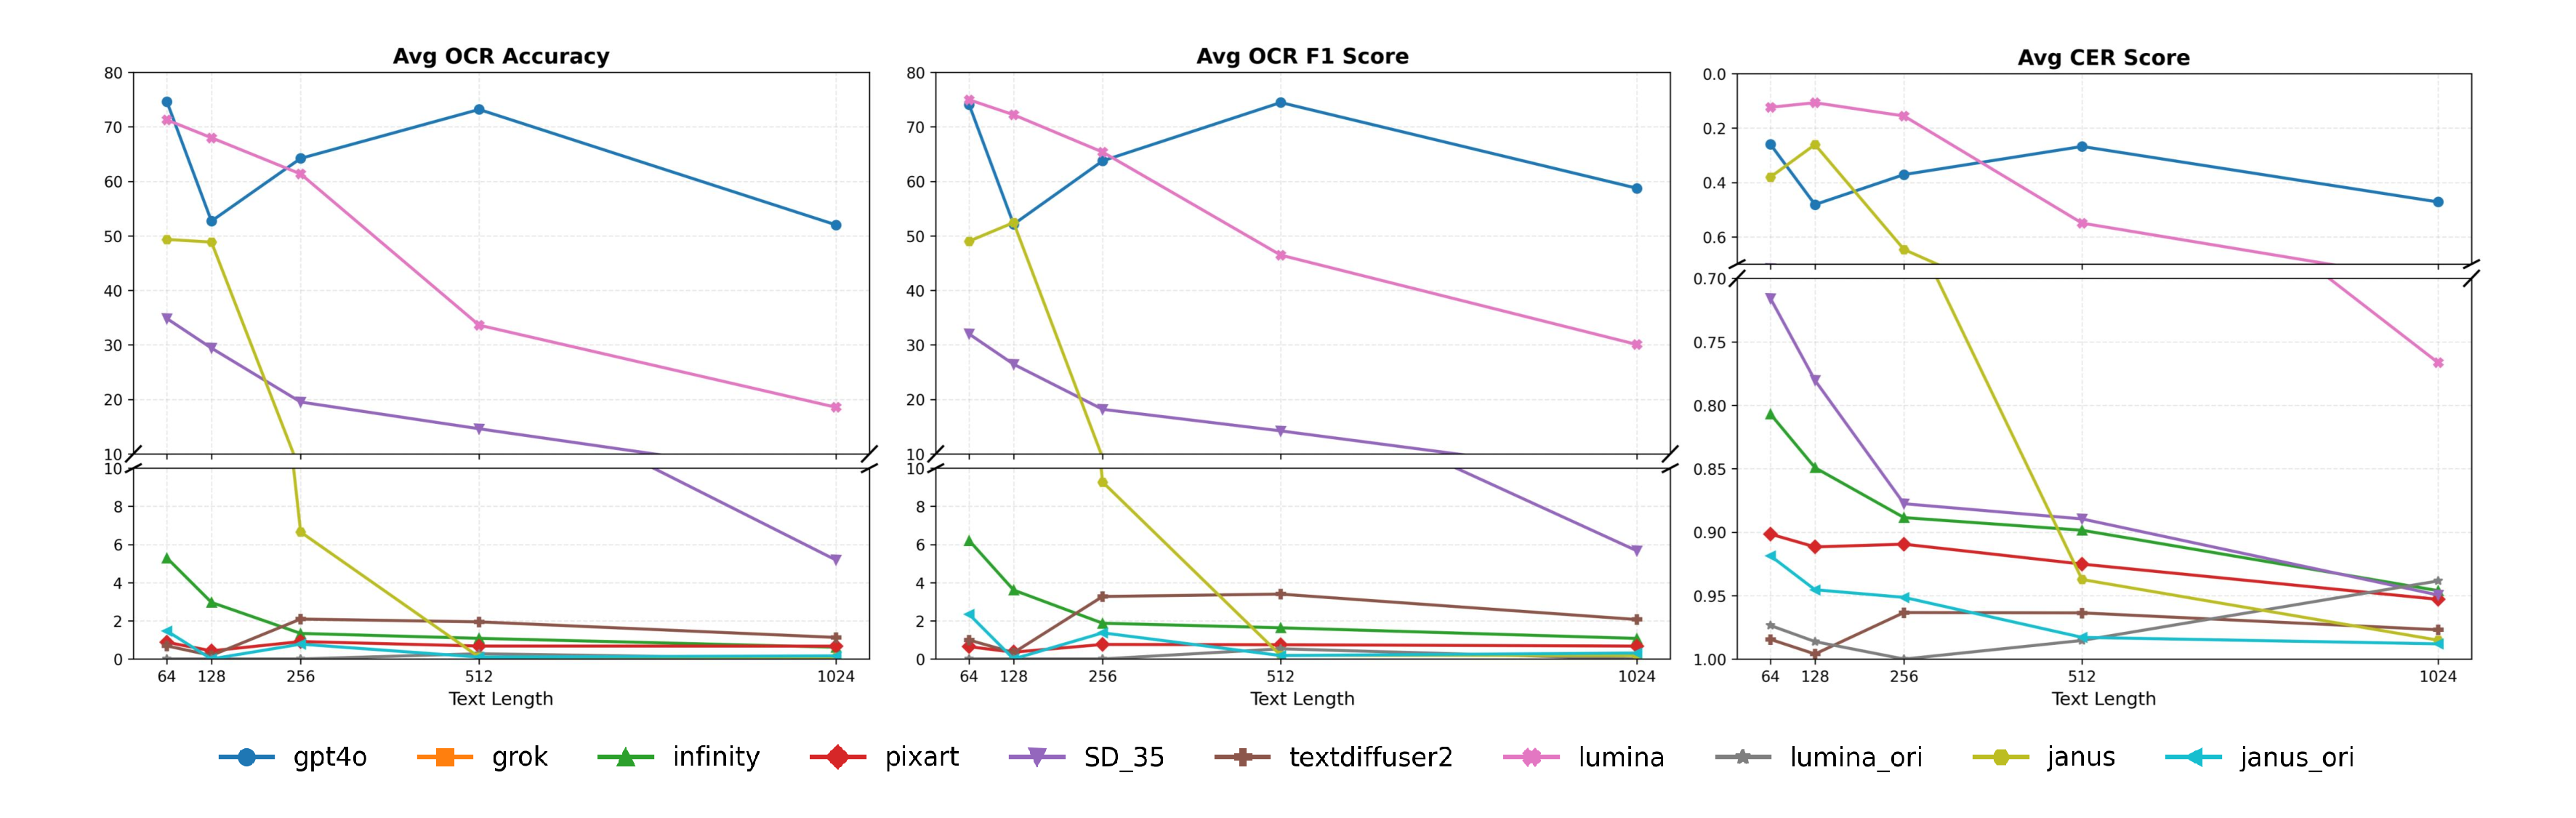
\includegraphics[width=1\textwidth]{Appendix/images/text_len.pdf}
    \caption{\textbf{OCR performance comparison of various models on the CleanTextSynth evaluation set across different text lengths. }We report average OCR Accuracy (left), F1 Score (middle), and Character Error Rate (CER; right, lower is better). Models \textit{Janus} and \textit{Lumina} represent our finetuned AR models, while \textit{janus\_ori} and \textit{lumina\_ori} refer to the original, unmodified models.}
    \label{fig:text_len}
\end{figure*}

We derive the following key observations:
Performance gains from dataset training: Both Janus-Pro-1B and Lumina-mGPT-7B show substantial improvements over their baseline versions when fine-tuned on our \DatasetName, highlighting the benefits of our data for text-centric generation tasks.
Length sensitivity: As expected, OCR accuracy significantly decreases with longer text sequences, indicating a persistent challenge in maintaining rendering quality at scale.
Competitive with GPT-4o: Our models outperform all open-source baselines and approach the performance of GPT-4o. Notably, in some cases, \textbf{our Character Error Rate (CER) is even lower than that of GPT-4o, further validating the effectiveness of our dataset in handling long-text scenarios}.



\subsection{Robustness Analysis on Short Sequences}

We provide a detailed analysis of how model performance varies with  short input text length from 2 to 64. 
Since the CleanTextSynth evaluation set lacks short-text cases, we additionally curated 140 samples from the interleaved Obelics dataset and constructed text variants ranging from 2 to 64 tokens. Each version was rendered using five representative models, including both open-source and closed-source systems. We employed Qwen2-VL as the OCR engine and computed standard recognition accuracy. 

\begin{table}[h]
\centering
\small
\caption{Recognition accuracy (\%) as token length increases. 
$^\dagger$ Model fine-tuned on TextAtlas5M.}
\begin{tabular}{c|cccccc}
\toprule
\bf Token Length & \bf AnyText & \bf TextDiffuser2 & \bf SD3.5 Large & \bf Grok3 & \bf GPT-4o & \bf Lumina-mgpt$^\dagger$ \\
\midrule
2  & 98.5 & 94.3 & 92.3 & 100.0 & 100.0 & 100.0 \\
4  & 94.3 & 92.2 & 89.4 & 100.0 & 100.0 & 100.0 \\
8  & 88.5 & 87.4 & 84.6 & 96.5 & 100.0 & 100.0 \\
16 & 47.3 & 61.5 & 78.3 & 93.2 & 100.0 & 98.4 \\
32 & 23.9 & 28.5 & 62.5 & 88.4 & 98.5 & 93.2 \\
64 & 17.4 & 18.9 & 45.3 & 76.5 & 96.7 & 85.7 \\
\bottomrule
\end{tabular}
\end{table}

We observe: \emph{i}. Performance of open-source models degrades sharply beyond 8–16 tokens. For example, TextDiffuser2 drops from 88.5\% at 8 tokens to only 11.5\% at 128 tokens.  
\emph{ii}. In contrast, GPT-4o and Grok3 exhibit strong robustness, maintaining accuracy above 76\% even for 64-token inputs. 

\paragraph{Conclusion.} 
This analysis highlights two critical insights: (i) most open-source models still struggle with rendering long or dense text, particularly beyond 10 tokens; and (ii) the primary cause is insufficient long-text supervision in prior datasets, which predominantly emphasize short, isolated words or captions. 
% We have added this quantitative study and its implications to the Appendix, thereby clarifying the bottlenecks of long-text image generation.



\subsection{Visualization of Generated Samples}

Figure~\ref{fig:lumina_mgpt_visualizatio} showcases representative samples generated by Lumina-mGPT after being trained on our \DatasetName. 
It is important to note that the \textbf{base model initially lacks any inherent text rendering capability}.

From the visualization, we observe the following:
Significant improvement in text rendering across all data types, indicating effective adaptation through our dataset.
Preservation of natural image generation quality, even in challenging scenarios such as realistic face synthesis—demonstrating that fine-tuning for text rendering does not compromise general visual fidelity.
These results highlight the strength of our dataset in enhancing text understanding while retaining high-quality image generation.

\begin{figure}[h]
    \centering
    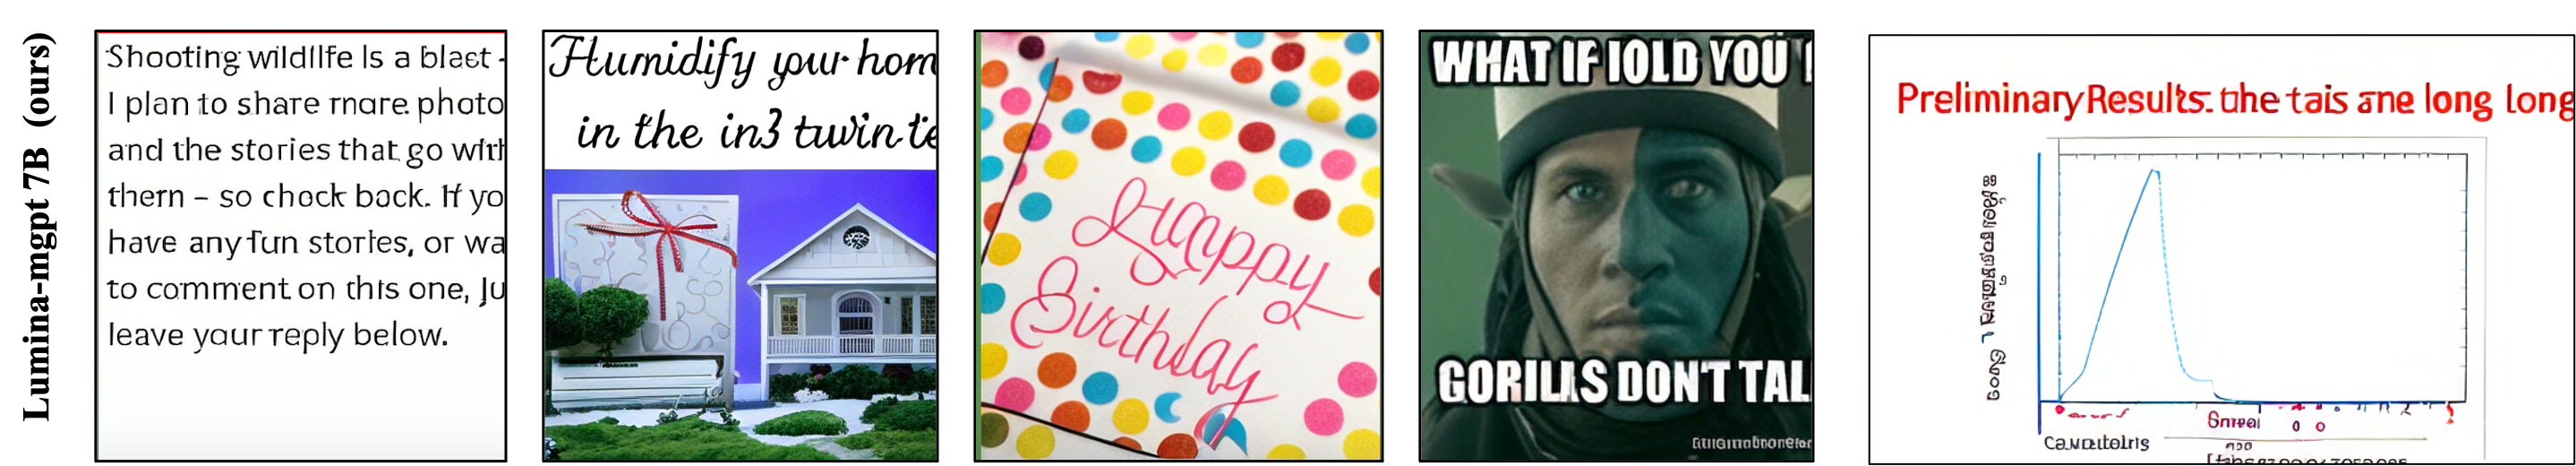
\includegraphics[width=\linewidth]{Appendix/images/7b_visualization.png}
    \caption{
    \textbf{Visualization of Lumina-mGPT (ours).}
The model shows significant improvements in text rendering while maintaining strong performance on challenging tasks such as realistic face generation.}
\label{fig:lumina_mgpt_visualizatio}
\end{figure}


\section{Autoregressive vs. Diffusion Models on Text Rendering}


\subsection{Tokenizer Has a Major Influence}
\begin{figure*}[h]
    \centering
    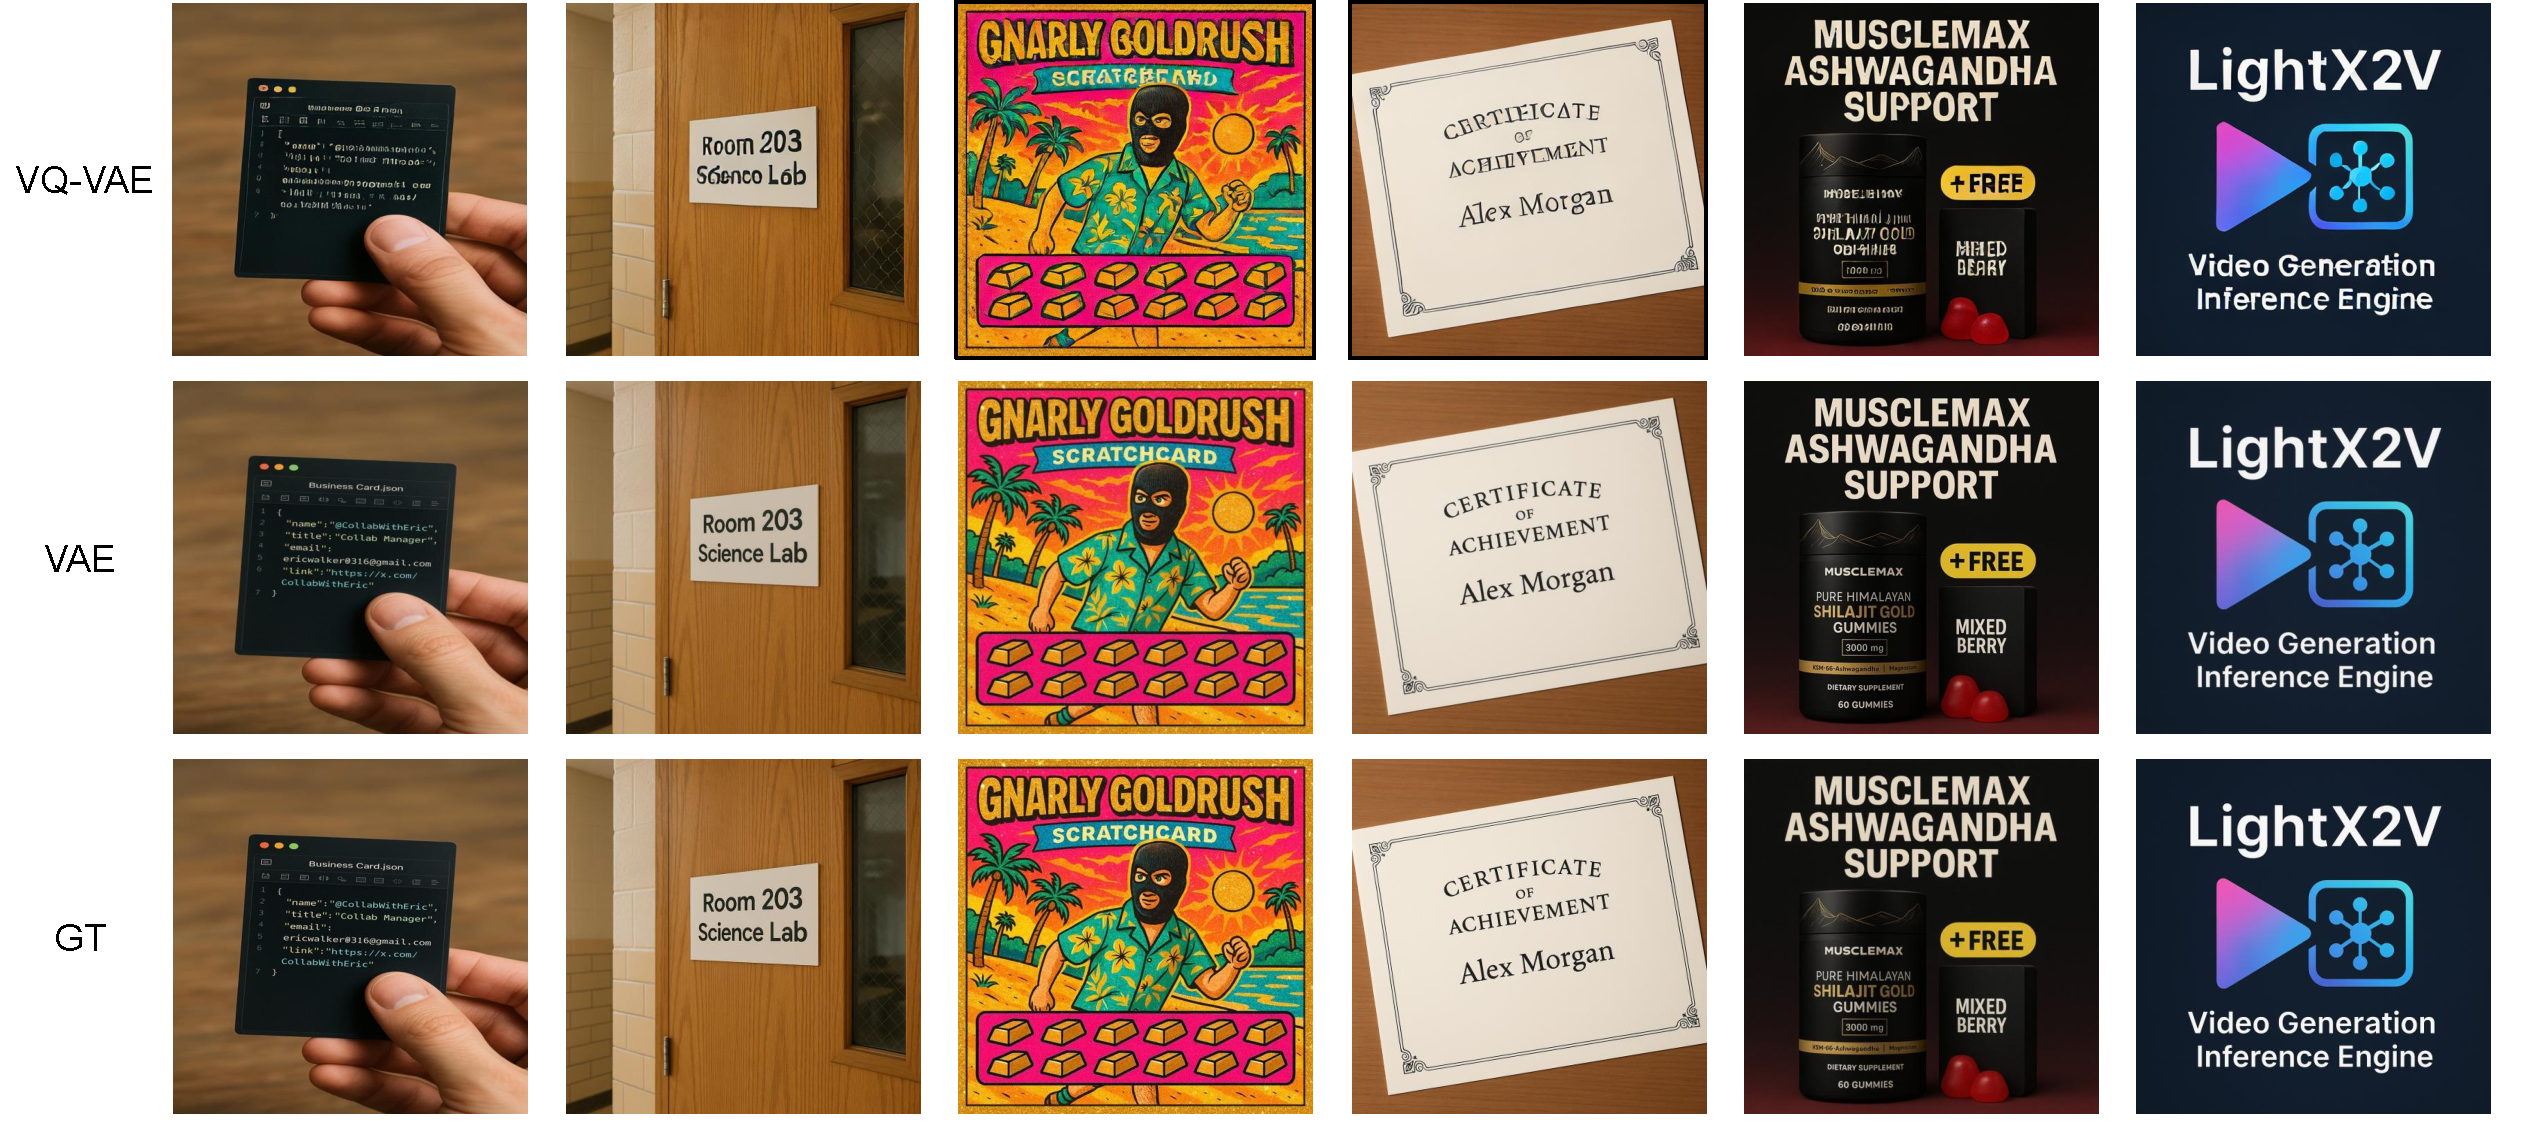
\includegraphics[width=1\textwidth]{Appendix/images/vq_vs_vae.pdf}
    \caption{\textbf{Comparison of image reconstructions across different generative tokenizers.} Each row corresponds to a different reconstruction method: VQ-VAE from Janus Pro~\cite{januspro}, VAE form Stable Diffusion 3.5 Large~\cite{sd3}, and ground truth. VQ-VAE struggles with fine-grained textual detail compared to the standard VAE Method.}
    \label{fig:vq_vs_vae}
\end{figure*}
In our training and evaluation, we observed that using VQ-VAE as a vision tokenizer notably impacts the performance of autoregressive generative models. Unlike VAEs, VQ-VAE quantizes continuous encoder features into discrete codebook entries, which introduces non-negligible information loss. This makes it challenging to reconstruct fine-grained visual details—such as small objects or complex structures—especially under low-resolution settings. To further examine this effect, we compare VQ-VAE tokenizer from Janus-Pro \cite{januspro} and VAE tokenizer from stable diffusion 
\cite{sd3} reconstructions at a fixed resolution of 512×512. As shown in Figure~\ref{fig:vq_vs_vae}, VQ-VAE struggles more with text fidelity and structural sharpness, reinforcing the limitations of discrete tokenization in preserving detail.

We further illustrate the resolution-dependent behavior of the Janus Pro's VQ-VAE tokenizer in Figure~\ref{fig:tokenizer}. As resolution increases, the model becomes more capable of reconstructing textual and structural details. For instance, at 256×256, certificate text and product labels are barely recognizable, while at 1024×1024, the reconstructions closely resemble the ground truth. However, this comes with a trade-off: the number of tokens grows quadratically with resolution, significantly increasing the computational burden for AR models. 

\begin{figure*}
    \centering
    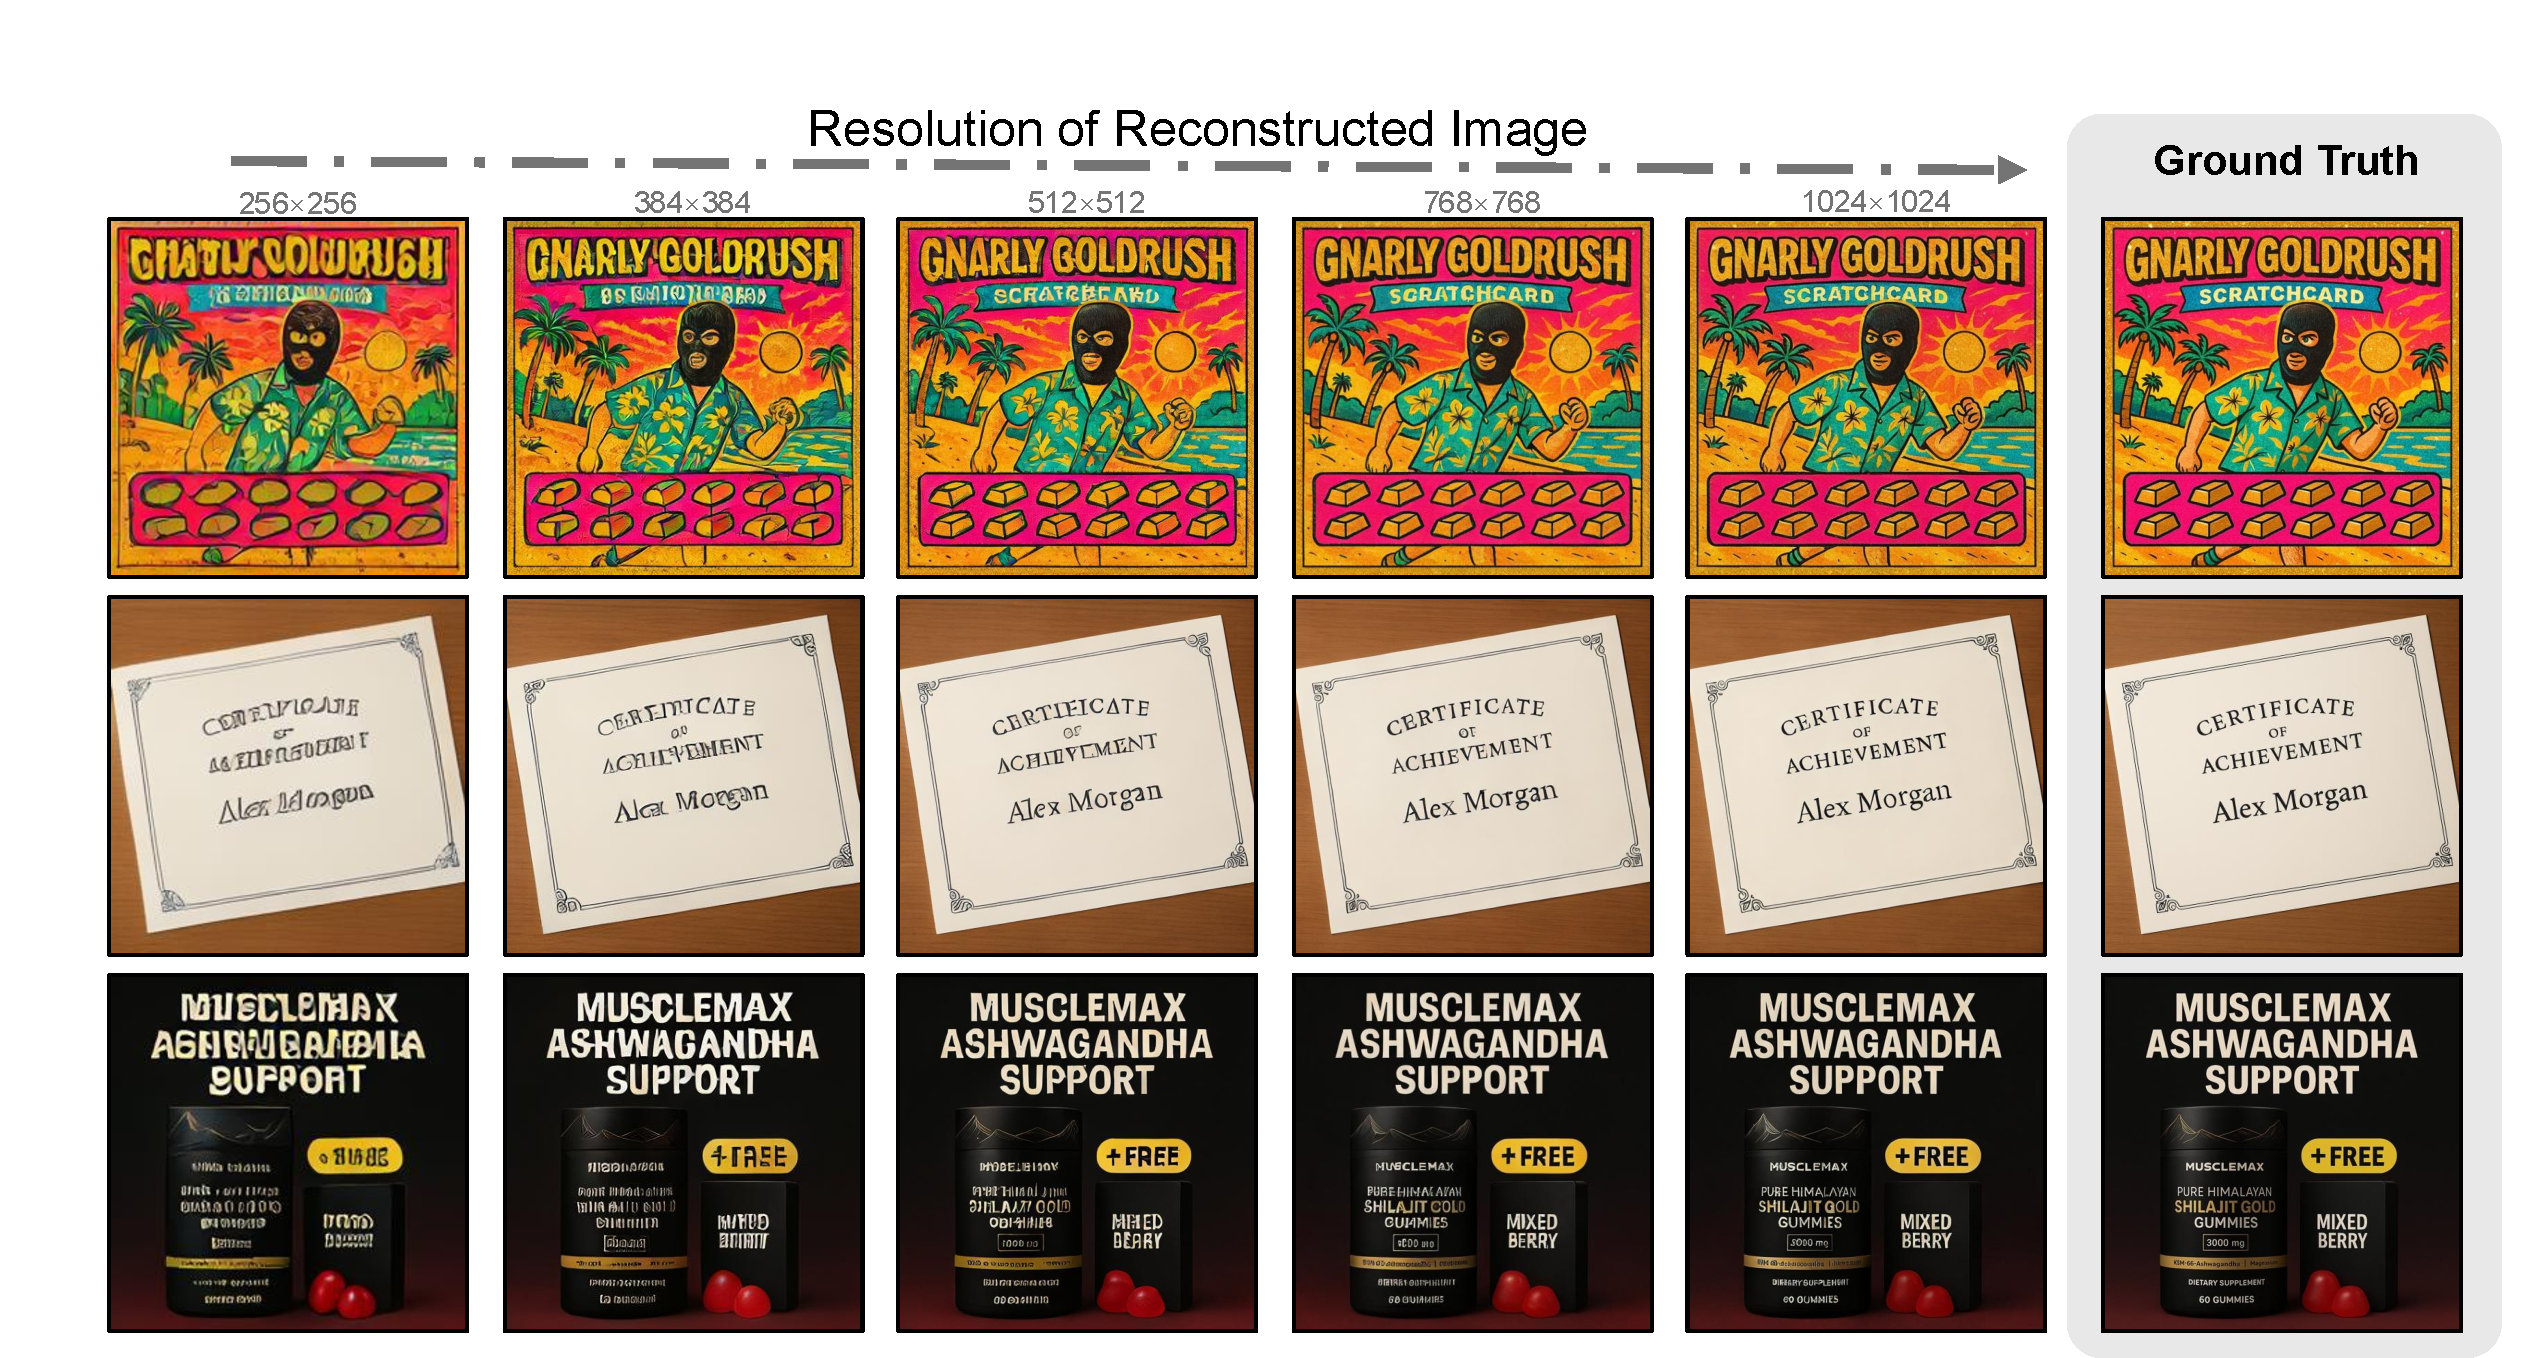
\includegraphics[width=1\textwidth]{Appendix/images/tokenizer_recon.pdf}
    \caption{\textbf{Reconstruction results of Janus Pro’s VQ-VAE tokenizer at increasing resolutions.} From left to right, image resolution increases from 256×256 to 1024×1024. Higher resolutions yield better reconstructions, especially in text clarity and layout fidelity. Ground truth (GT) images are shown in the final column for reference.}
    \label{fig:tokenizer}
\end{figure*}


\subsection{Generation result comparison}
In this section, we compare the text rendering capabilities of our diffusion-based model PixArt-$\alpha$ with the autoregressive model Lumina-mGPT, both trained on our proposed dataset, \DatasetName.

For the diffusion model, we evaluate two types of prompts:
(1) “Generate an image of size $512 \times 512$ according to the following prompts: xxx”, and
(2) “A billboard outdoors with text: xxx”.

The qualitative results are presented in Figure~\ref{fig:ar_vs_diffusion}. Our key observations are as follows:

\begin{itemize}
\item \textbf{Detail rendering:} The diffusion model excels in visual fidelity, even at a resolution of $512 \times 512$. It produces well-formed and accurately aligned text. This advantage is largely attributed to its use of continuous token representations, which offer finer granularity than discrete tokens used in autoregressive models.

\item \textbf{Textual coherence:} The autoregressive model demonstrates superior coherence in word sequence and correctness of generated content. However, its visual rendering is less precise—words often appear loosely structured or distorted. We attribute this to the nature of autoregressive decoding, which focuses on sequential word prediction rather than global image consistency.

\item \textbf{Layout consistency:} While diffusion models render text sharply, they occasionally introduce hallucinated or irrelevant text, especially in complex layouts. This inconsistency reflects the model’s weaker control over semantic alignment in dense text scenarios.
\end{itemize}



\begin{figure}
    \centering
    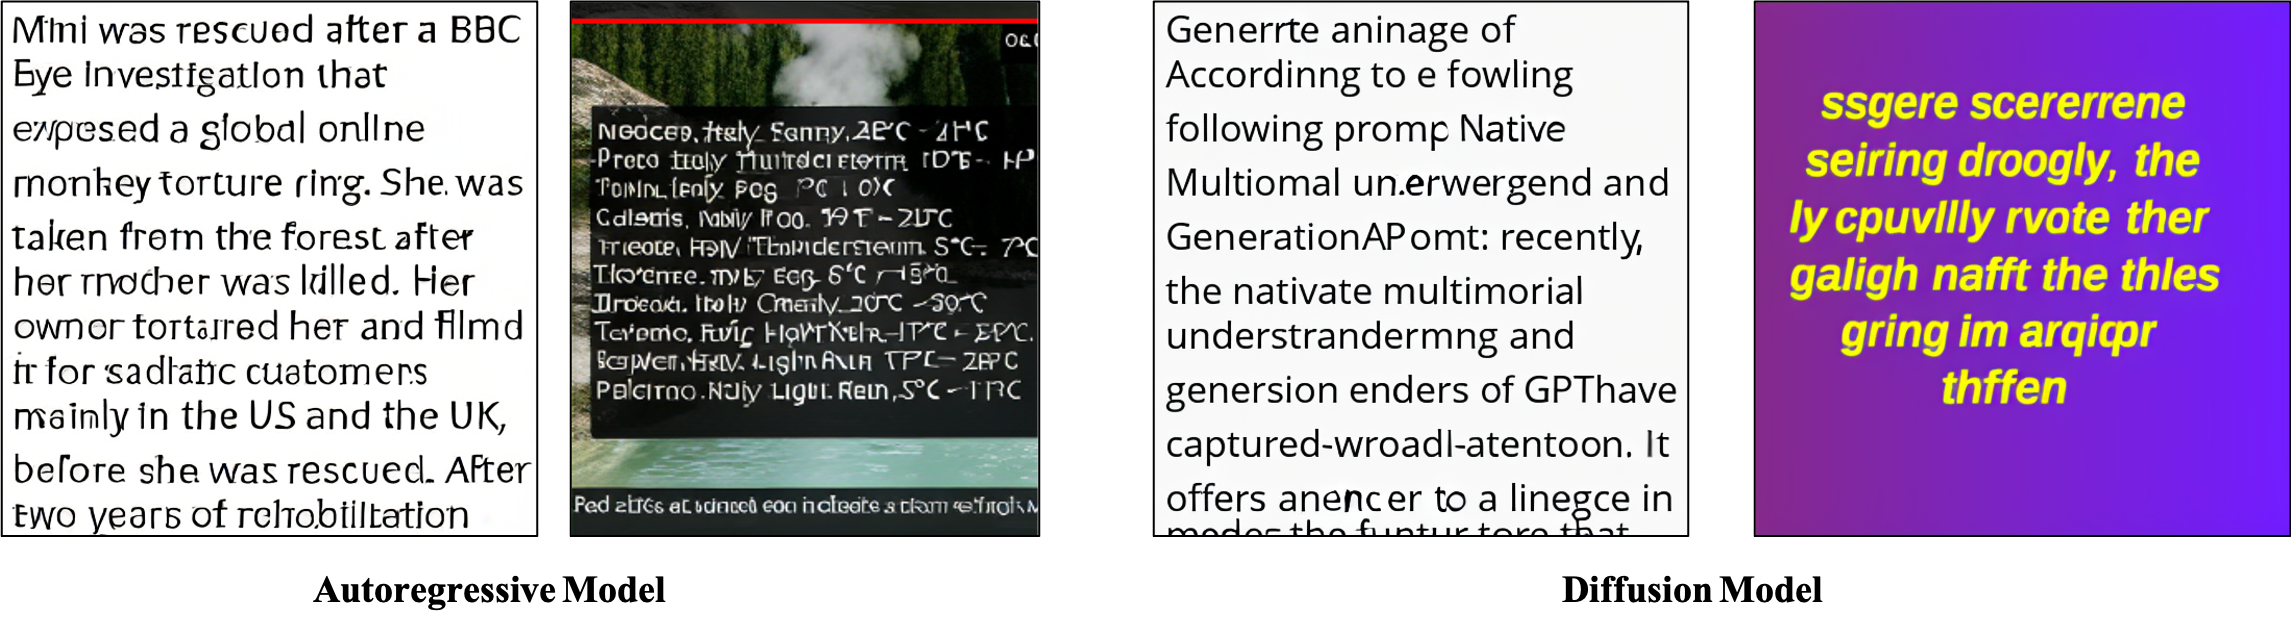
\includegraphics[width=\linewidth]{Appendix/images/ar_vs_diffusion.png}
    \caption{
    \textbf{Comparison between autoregressive and diffusion models} for text-to-image generation at $512\times512$ resolution.
    While diffusion models yield finer visual details, autoregressive models demonstrate stronger output consistency.
    }.
    \label{fig:ar_vs_diffusion}
\end{figure}


% \section{Cross domain evaluation.}




% \input{tables/topic_dataset}


\section{Visualization}


\subsection{Layout Planning Comparison}
It is worth noting that although SD-3.5~\cite{sd3} Large significantly outperforms PixArt~\cite{pixart} and Infinity~\cite{han2024infinity} in OCR-related scores on the TextVisionBlend subset, its FID and CLIP scores are lower than those of the other two models. To better understand this phenomenon, we present two representative cases in Figure~\ref{fig:special case}, analyzing the differences in model performance on this subset.

In the first row of Figure~\ref{fig:special case}, SD-3.5 fails to capture the interleaved image layout and does not render text well, whereas both Infinity and PixArt follow the interleaved structure and white-background requirement, despite their poor text quality. This may explain SD-3.5’s lower CLIP and FID scores. Meanwhile, in the second row, all three models exhibit interleaved characteristics, but only SD-3.5 generates relatively complete text in the image. This likely contributes to its strong OCR-related performance.

Overall, when generating images with complex requirements, SD-3.5 performs poorly in terms of image layout and certain specifications. We speculate that this may be related to the model's supported input text length. PixArt-Sigma can accommodate up to 300 text tokens, while Infinity, as an autoregressive generation model, supports even longer text inputs. A greater text input capacity may provide an advantage in understanding complex instructions.


\subsection{Comparison of Existing Models on \EvalDatasetName}

We present a comparative analysis of existing text-to-image generation models in Figure~\ref{fig:sota_performance}.
Among all models, GPT-4o significantly outperforms others across all subsets of \EvalDatasetName, demonstrating a substantial lead in both visual quality and text fidelity. Grok3 also shows strong performance, yet the gap between closed-source and open-source models remains considerable.

Notably, with the introduction of our benchmark dataset, \EvalDatasetName, we observe a noticeable reduction in this performance gap—highlighting its effectiveness in driving progress and bridging disparities between different model families.

\begin{figure}
    \centering
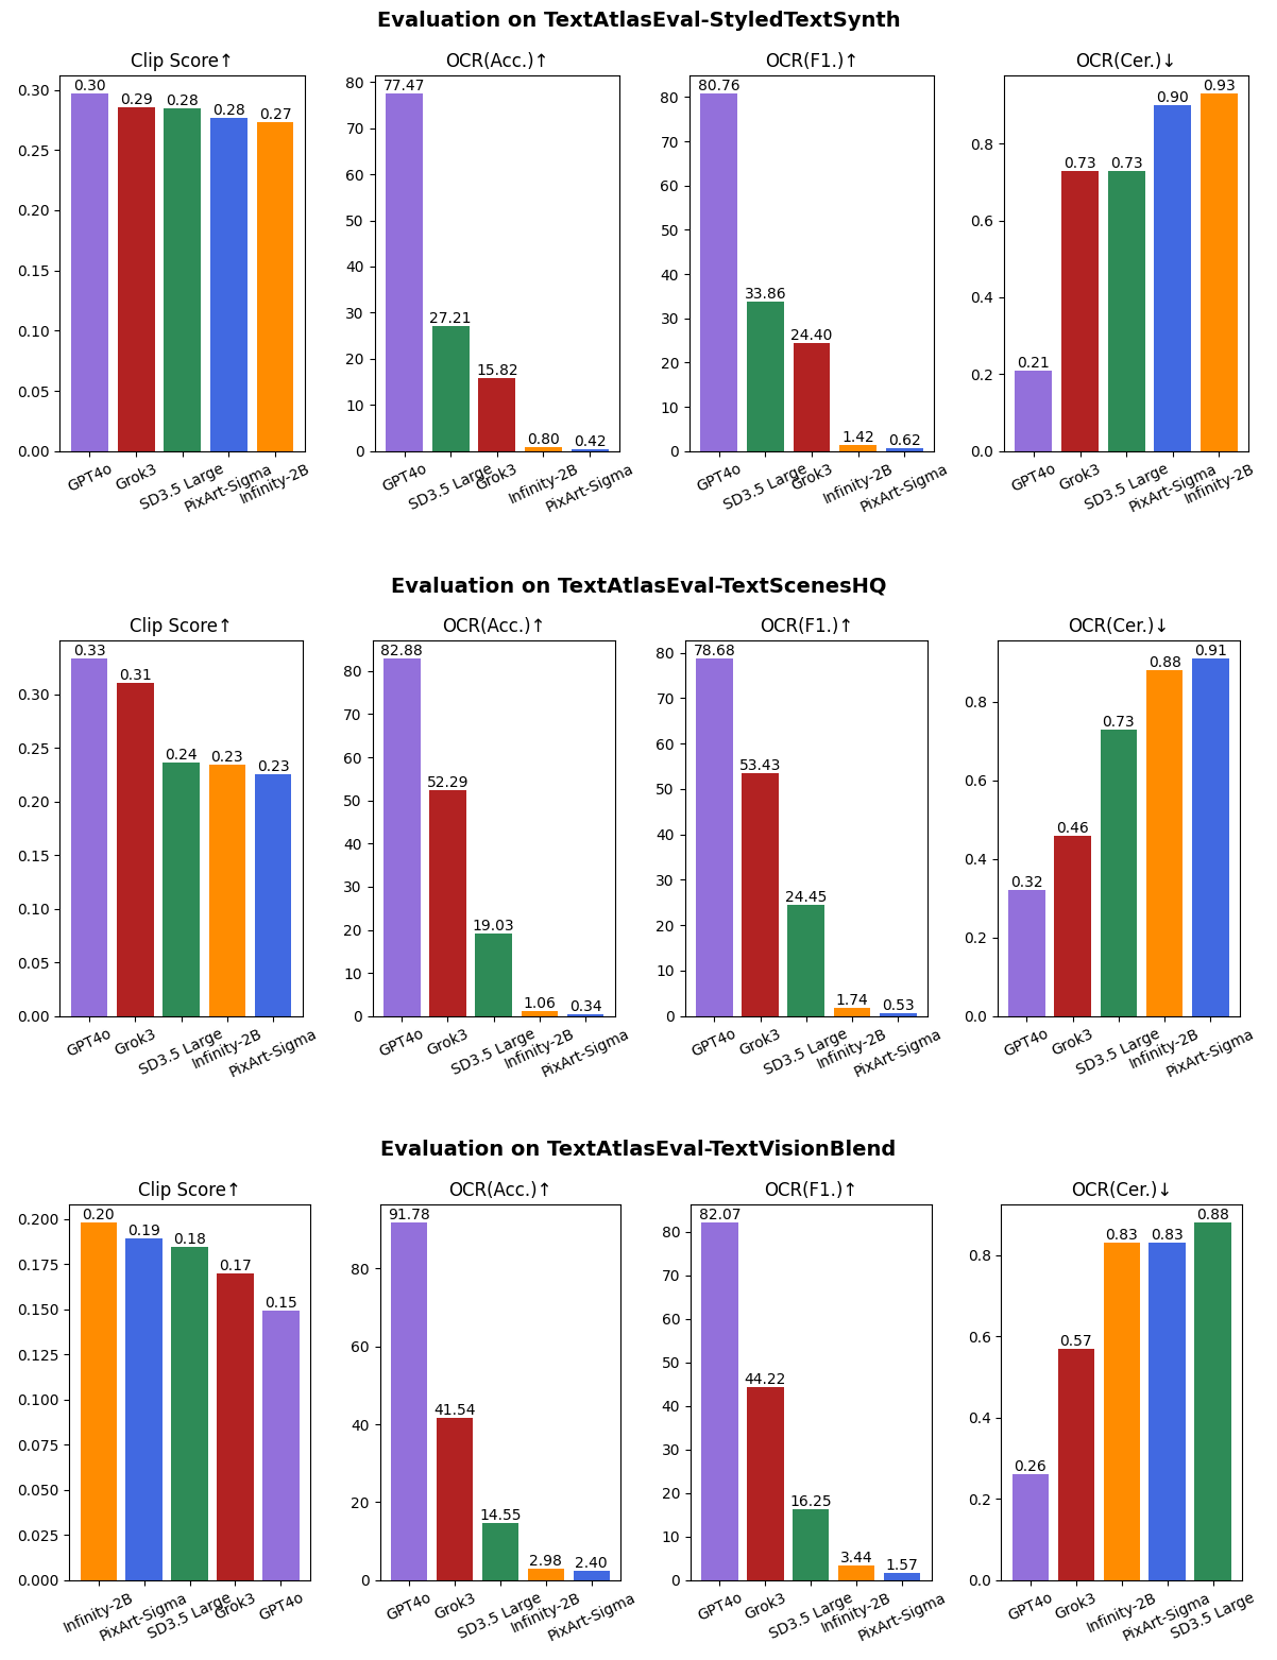
\includegraphics[width=\linewidth]{Appendix/images/performance_comparison.png}
    \caption{Performance comparison of state-of-the-art text-to-image generation models on our proposed benchmark, \EvalDatasetName.}
    \label{fig:sota_performance}
\end{figure}

\input{figures/result_special_case}

% \section{LDA Topic Analysis.}


% \subsection{More visualization of our customed trained model}
% In this part, we show more samples.
% We observed, notice that the base Lumina-mgpt model has no rendering ability at all.
% The model trained on our dataset shows .
% This indicates our dataset improve the text rendering .


\section{Creation of the Synthetic Dataset}
\label{sec:appendix_create_synthetic}
\subsection{Creation of StyledTextSynth}
\label{sec:appendix_create_mq}

\subsubsection{Text Prompt for StyledTextSynth Image Generation}
\paragraph{General Prompt:}
The core of the synthetic data involves utilizing text-conditioned image generation methods. 
For simple topics like billboards, we follow a "General Prompt" approach with the following guidelines:
\begin{itemize}
    \item Provide a reasonable description of the billboard.
    \item Ensure the billboard faces the camera directly.
    \item The billboard should occupy at least one-third of the image.
    \item Incorporate a complex background for added detail.
    \item Keep the billboard's color consistent, with no additional context.
    \item Limit the total text on the billboard to fewer than 160 words.
    \item Ensure the billboard is visible, vehicle-related, and not overlapped by other objects.
\end{itemize}

We show an example in Table~\ref{tab:mqcallgpt4o}, with detail instruction the LLM generate reasonable scene description for image generation model.

\input{Appendix/tables/mq_call_gpt4o}



\paragraph{Topic with Human-Designed Seeds:}
Certain topics, such as \textit{studio} scenes, can involve highly complex setups. 
To address these challenges, we simplify the generation of text regions by incorporating human-designed seeds. 
Specifically, the instructions include a \textit{general prompt} combined with a predefined, human-curated scene to serve as the seed, ensuring better coverage and control over these intricate scenarios.

\begin{itemize}
    \item Weather Report: A host stands in a studio, with a display screen behind them showing weather conditions for various locations. In the foreground, a white rectangular box occupies one-third of the screen.
    \item TV Shopping: A host stands beside a table, holding a product in their hand, with an advertising board placed vertically next to them.
    \item Instruction Manual: An instruction manual is placed vertically, with objects associated with it positioned nearby.
\end{itemize}


\paragraph{Template Topics with Fixed Text Region Position}:
Some topics can be used as template to generate more samples, what is different is that the text appeared position is fixed.
For these generate samples, we can simply generate more samples by simple text replace.

\begin{itemize}
    \item News: Describe an image that could appear on television news. It can depict either positive or negative events, with diverse content. The total word count should be less than 160 words.
    \item Cinema Poster: Describe an image of a movie poster. It can be of any genre. The total word count should be less than 160 words.
\end{itemize}


\input{Appendix/tables/mq_text_call_gpt4o}

\input{Appendix/tables/mq_text_call_llama}


\input{Appendix/tables/mq_text_call_qwen}

\subsubsection{Utilizing LLMs for Text Generation in Specific Scenes}


After generating scene images without text, it is necessary to call upon an LLM to create contextually relevant sentences for rendering. 
To ensure realism in the generated outputs, we employ \textbf{Scene-Dependent Text Generation}. 
For general topics, such as noticeboards, we prompt the LLM to produce sentences based on the given topic. 
Examples of such outputs are shown in Table~\ref{tab:mq_text_call_gpt4o} and Table~\ref{tab:mq_text_call_llama}.
The LLMs accurately generate text appropriate for the given scene.


\paragraph{Visual-Dependent Scenes:}  
In some cases, the visual appearance of the scene is closely connected to the text and requires fine-grained visual understanding. 
For instance, a generated poster with rich visual elements may need text that complements its design. 
In such scenarios, we use LVM models that process both text and image inputs to produce reasonable outputs. 
An example of this process is shown in Table~\ref{tab:mq_text_call_qwen2}.
By incorporate specific instruction, the model produce reasonable output.



\subsubsection{How Do We Select Data Topics for Rendering?}
Originally we generate 50 topics that include dense text, one more question is how to filter these topics.
With this in mind, we design the following filter rules:
\begin{enumerate}
    \item \textbf{Avoid topics directly tied to font generation}, such as store signs, wayfinding signs, or on-screen text.
    \item \textbf{Exclude topics where the renderable area is too small}, such as mobile phone screenshots.
    \item \textbf{Avoid topics with unclear boundaries or artistic fonts that are hard to recognize}, such as neon signs.
    \item \textbf{Prioritize topics with better rendering results in SD3.5 over similar ones}, e.g., choose "digital display" over "OLED display" or "banner" over "protest marches."
\end{enumerate}



\subsubsection{Text Deduplication in StyledTextSynth Data}
The text in the synthetic data is generated by Llama 3.1, GPT4o, and Qwen2VL. 
In most topics, there is basically no obvious disharmony between the generated images and the scenes, so we mainly use the text generated by Llama 3.1 and GPT4-o. 
For some scenes where the images and texts are highly correlated, VLM is needed to generate texts that match the image content.
Under the same or semantically similar topics, there may be semantic duplication. To this end, we semantically deduplicate the generated text based on the sentence-transformers library. 

\paragraph{Deduplication Process with Semantic Hashing}
The deduplication process consists of the following steps:
\begin{enumerate}
    \item \textbf{High-Dimensional Semantic Representation:} 
    Obtain the high-dimensional semantic representation of the text.

    \item \textbf{Dimensionality Reduction:}
    Map the high-dimensional semantic vector to a fixed low-dimensional space using random projection.

    \item \textbf{Semantic Hash Generation:}
    Generate semantic hashes based on the projection results.

    \item \textbf{Pairwise Similarity Comparison:}
    Use Hamming similarity to perform pairwise comparisons of the semantic hashes. A Hamming similarity threshold of 0.9 is applied to detect and remove semantically similar texts.

\end{enumerate}

This structured approach ensures effective and accurate text deduplication while maintaining semantic integrity.


\subsubsection{Middle-Quality Sample Filtering}

To enhance the quality of the generated middle-quality samples, we apply a set of filtering rules to reject unsuitable samples. The primary criteria for rejection are as follows:

\begin{itemize}
    \item Insufficient areas available for rendered text.
    \item Excessive similarity to other topics, reducing diversity.
    \item Difficulty rendering text in curved areas.
    \item Unrealistic or artificial appearance of the image.
    \item Challenges in identifying or defining bounding boxes.
    \item Presence of incorrect or irrelevant text.
    \item Poor recognition quality or unclear visual details.
\end{itemize}

Examples of rejected samples are illustrated in Figure~\ref{fig:mq_reject_sample}.

\input{Appendix/mq_rejected_samples}


\subsection{Gen Interleaved Data Benchmark}
\label{sec:interleave}
The process of generating interleaved data is divided into three main parts: data selection, PDF generation, and annotation generation.
% \textcolor{red}{We select from WIT and OBELICS}.
\subsubsection{Data Selection}
We select data from WIT~\cite{wit} and OBELICS~\cite{obelics}. 
The WIT dataset contains samples from Wikipedia, with each sample comprising an image and multiple associated text segments, such as titles, main text, subtitles, subtext, and image captions. From this dataset, we sample instances containing a single image and interleaved text. 
The OBELICS dataset consists of interleaved image-text documents sourced from web pages in the Common Crawl. Each OBELICS sample includes multiple images with their corresponding text segments. For our purposes, we sample data containing two to four images to maintain manageable image sizes. 
Finally, we sampled 69.8\% data from the WIT and 30.2\% data from the OBELICS, respectively.
\subsubsection{PDF Generation}
After selecting the data, we use the PyMuPDF~\cite{pymupdf} library to generate parseable PDF files based on the sampled data. To accommodate the two types of data, we design different layout generation strategies according to their respective structures.

For both datasets, the layout strategy involves first randomly assigning image positions on the page, followed by allocating text boxes in a manner that optimally utilizes the remaining space. For the WIT dataset, since the text segments have predefined types (e.g., title, main text, subtitle), we impose additional constraints to ensure structural consistency. For instance, titles are placed at the top of the corresponding image to maintain semantic alignment. In contrast, for the OBELICS dataset, we adopt a simpler approach where the text boxes are sequentially assigned in a top-left to bottom-right order across the layout.

To implement the layouts, we use the  \texttt{insert\_htmlbox()}  from PyMuPDF to insert images and text into the PDFs. The font for each sample is randomly selected to introduce variation. To further standardize the generated PDFs, we limit the text in each text box to a maximum of 50 words. Additionally, after generating the PDFs, we save a rendered image version of each page to serve as the corresponding image data for our dataset.


\subsubsection{Annotation Generation}
After generating parseable PDFs, we use the PyMuPDF to extract information such as the bounding boxes of text and images, as well as text font sizes and styles. Additionally, we utilize Qwen2-VL to generate captions for each image within the PDF. The prompt used for caption generation is: "\texttt{Generate the caption of the image, and the caption should be no more than 50 words.}"

Finally, we obtain detailed information for the text, including its content and bounding boxes, along with the captions and bounding boxes of the images. By combining these elements based on the generated template, we produce the interleaved data annotations.

\subsection{Template Generation Details}
\label{sec:appendix_template_details}

\input{Appendix/tables/call_gpt}

To create templates for summarizing descriptions and text, we utilized an LLM to generate a total of 600 templates. The prompt used for this process is detailed in Table~\ref{tab:template_generate}.



\subsection{Bounding Box Annotation and Detector Training  for StyledTextSynth Sample}

\subsubsection{Bounding Box Generation}

\begin{enumerate}
    \item \textbf{YOLO Results:} Based on the model's output, select the bounding box with the largest rectangular area when multiple results are present.
    \item \textbf{Fine-tuned RT-DETR\_R50VD Results (Packing Box):} Use the model's output to identify the bounding box. If multiple results are present, select the one with the smallest difference between width and height.
    \item \textbf{RT-DETR\_R50VD Results (Booklet Page):} Check if the output contains the label "book". If multiple results are present, choose the bounding box with the smallest width-to-height difference.
\end{enumerate}

For all three methods above, the results are passed through SAM2 (Segment Anything Model v2) to refine recognition. The SAM2 output is converted into center points to serve as prompts, improving predictions for slanted surfaces.

\subsubsection{Detector Training}

\paragraph{YOLO Training Process:}

\begin{enumerate}
    \item For each topic (excluding template topics like Alumni Profile and News, as well as rejected topics), start with the YOLOv11l initial weights and manually label about 1,000 failed detection samples. Use the following annotation methods:
    \begin{enumerate}
        \item For slanted images, use the \texttt{labelme} tool to annotate with quadrilateral bounding boxes (four points).
        \item For upright images, annotate using the \texttt{Code} tool with two points (top-left and bottom-right).
    \end{enumerate}
    Annotate areas of the image where the topic is unobstructed, and convert all annotations to YOLO format with the class label set to 0.
    \item Train the model on the mixed annotated dataset for approximately 400 epochs (or more) to obtain initial weights.
    \item Test the initial weights on each topic. A detection rate of at least 40\% is considered usable for that topic.
    \item For topics with low detection rates in Step 3, augment the manually labeled dataset for that topic with approximately 1,000 additional images. Apply transformations such as scaling, composition, flipping, and affine transformations. Combine the augmented data with the original manually labeled data (totaling approximately 2,000 images), and retrain the model for an additional 200 epochs.
    \item Certain topics may share weights based on detection performance. For example:
    \begin{itemize}
        \item \textbf{Billboard} and \textbf{TV Shopping} can share the same weights.
        \item \textbf{Blackboard Classroom} and \textbf{Advertisement Poster} can share the same weights.
    \end{itemize}
\end{enumerate}

\paragraph{Fine-Tuned RT-DETR\_R50VD Training:}

\begin{enumerate}
    \item Fine-tune the RT-DETR\_R50VD model specifically for the \textbf{Packing Box} topic. Use 1,000 manually annotated packing box samples from Step 1.
    \item Train the model  for approximately 100 epochs.
\end{enumerate}




\subsection{Text Rendering Details}

\subsubsection{Bbox Text Rendering:}
After obtaining images generated by Stable Diffusion and images from CommonCrawl, which contain large fillable text areas (such as billboards, electronic screens, etc.), we use YOLO v11 and RT-DETR\_r50vd to identify and label the fillable areas in the images. However, these detectors can only recognize rectangular areas, and the labeled fillable regions are often slightly larger than the actual fillable areas. 
Therefore, we further use SAM2, starting from the center point of the bounding box, to search for color-matching areas. This ensures that the new bounding boxes generated by SAM2 more accurately cover the fillable areas, breaking the traditional rectangular limitation and supporting the detection and filling of irregular quadrilaterals.

For text content generation, we use Llama-3.1-8B, GPT-4o, and Qwen2-VL-7B. 
Among them, Qwen2-VL-7B is mainly used for generating text related to cinema posters.

\textbf{Rectangular Bbox Text Rendering}
For detected rectangular bounding boxes, we directly render text within the area. 
The font is randomly chosen from 10 common fonts, and the font size is automatically adjusted based on the bounding box size to fill the area as much as possible, ensuring both aesthetics and readability.

\textbf{Irregular Quadrilateral Bbox Text Rendering}
For detected irregular quadrilateral bounding boxes, we first create a transparent layer and render the text on that layer. Then, we use a perspective transformation to adjust the transparent layer to match the irregular quadrilateral shape of the bounding box and finally composite it onto the original image, ensuring the text accurately fits the fillable area.

\subsubsection{Template Rendering Method: }
For images related to News Shows, Weather Reports, and Cinema Posters, where text usually appears in relatively fixed areas, we use a template rendering approach for text filling. We create background templates for these topics based on real-world images, label the fillable areas of the templates with bounding boxes, render the background templates onto the original image, and then fill the text according to the bounding box annotations of the templates.



% \clearpage


\section{Creation of the Real Dataset.}
\label{sec:appendix_create_real}

\subsection{Data Selection Details from Existing Datasets}
\label{sec:appendix_data_selection}
To ensure the quality of selected samples, we apply a rigorous filtering pipeline consisting of the following steps:

\begin{enumerate}
    % \item \textbf{English-Like Check:}  
    % Text is evaluated for resemblance to English. At least 70\% of the words must contain alphabetic characters to ensure alignment with natural English patterns.
    
    \item \textbf{Minimum Length Check:}  
    Samples with fewer than seven words are excluded. This criterion eliminates excessively short texts that may lack meaningful content.
    
    \item \textbf{Unique Word Ratio Check:}  
    To promote diversity, the ratio of unique words to total words must exceed 0.3. Samples with overly repetitive word usage are filtered out.
    
    \item \textbf{Consecutive Repetition Check:}  
    Text containing more than three consecutive repetitions of the same word is excluded to prevent redundancy and improve coherence.
    
    \item \textbf{Word Validity Check:}  
    Each word must include at least one alphabetic character and be longer than one character. This ensures all words are meaningful and eliminates noise or random symbols.
    
    \item \textbf{Text Cleaning:}  
    Non-alphanumeric characters, except spaces, are removed. Multiple spaces are normalized into a single space to ensure the text is clean and consistently formatted.
    
    \item \textbf{Annotation Sorting:}  
    Annotations are ordered spatially, following a top-to-bottom and left-to-right sequence based on the coordinates of bounding polygons. This ensures spatial coherence in the text layout.
\end{enumerate}

This pipeline is designed to refine the dataset and maintain high standards for text quality and diversity.


\subsection{Extracting Powerpoint Data}
We extract the powerpoint data with PyMuPDF~\cite{pymupdf}.
Specifically, we transform the each page of powerpoint into pdf format, then we rephrase the powerpoint data by blocking description.
For example, it split the all page into different block.
Each block include elements like text or image, for text element we extract the word and for image we use the QWen-VL to generate caption and the prompt is simple \textit{Describe this image}.
For example, we simply call image.


\subsection{PPT2Details annotation generation.}
In the PPT2Details subset, we use Qwen2-VL to summarize all extracted elements (text, figures, layout, etc.) into a single descriptive prompt.
The text prompt for calling Qwen2-VL is:
\begin{tcolorbox}[title=Prompt Format]
Given a PowerPoint slide image, extract and summarize all visual elements—such as text blocks, charts, tables, and diagrams—into a single, fluent, and logically consistent paragraph. 

You must:  
1. Accurately preserve all textual content and wording details.  
2. Include descriptions of all visual elements (e.g., diagrams, tables) if present.  
3. Avoid omitting or paraphrasing key phrases.  
4. Output only one paragraph per slide.
\end{tcolorbox}
% "Given a PowerPoint slide image, extract and summarize all visual elements—such as text blocks, charts, tables, and diagrams—into a single, fluent, and logically consistent paragraph. You must:1. Accurately preserve all textual content and wording details. 2. Include descriptions of all visual elements (e.g., diagrams, tables) if present. 3. Avoid omitting or paraphrasing key phrases. 4. Output only one paragraph per slide."


\subsection{Data Selection Details for TextScenesHQ Dataset}
After crawling images according to topics, we use the easyOCR\footnote{https://github.com/JaidedAI/EasyOCR} library to recognize the text in the images. 
First, we save images containing more than 10 words, and then organize the text information from the upper left to the lower right to construct a JSON file. 
The content of the JSON file includes the text and its corresponding bounding box.
During this process, some difficult data may have spelling errors, including but not limited to confusion between numbers and letters, spelling errors, and capitalization errors. 
In this regard, we use Llama 3.1~\cite{llama3h} to check and correct the recognized text to improve the accuracy and quality of the text.



\subsection{TextScenesHQ Image Filtering}
For real image data, we primarily discarded samples where the text was not clearly visible. 
Additionally, samples were rejected if the detected text contained too few words (fewer than 10 in this study).
We show the rejected samples in Figure~\ref{fig:hq_reject_sample}.

\input{Appendix/hq_rejected_samples}


\subsection{TextScenesHQ Image Annotation}
\label{sec:appendix_textsceneshq_annotation}
After using OCR for filtering and generating bounding boxes around the text in the images, we convert the detected Chinese text and its corresponding bounding boxes into a text JSON format. Due to the diversity and complexity of the images, OCR results may contain spelling errors and misordered text. To address this, we perform three corrective steps using Llama 3.1 and Qwen 2.5-Coder. First, Llama 3.1 is used to correct any spelling mistakes in the text. Next, we use Llama 3.1 to reorder the text slightly to align with the proper syntax, as OCR typically outputs text in a left-to-right, top-to-bottom sequence without considering the multi-column layout in the images. After reordering, we generate the corrected text JSON. The third step involves addressing any potential formatting issues in the JSON. If the JSON generated in the second step is not parsable, we use Qwen 2.5-Coder to output the text JSON in markdown format to ensure proper structure.

For the image background descriptions, we use Qwen 2.5-VL to generate contextual information while preventing it from outputting any descriptions of the text within the image. Additionally, we created 500 diverse and complex scenario templates using GPT-4o to generate a wide range of image descriptions. These descriptions, combined with the corresponding text JSON, are used to generate comprehensive image information in JSON format.


\subsection{Quality classification}
In this work, we mainly split the data quality according to the visual appealing semantic, and if the image include dense text and have correct captions.

% \textcolor{red}{\textbf{Plot Some powerpoint data}.
% Specifically, we plot some cases with or without images. 
% Ensure more diversity.
% }


% \clearpage

\section{Annotation Details}



% \begin{wrapfigure}{r}{0.5\linewidth}
%     \centering
%     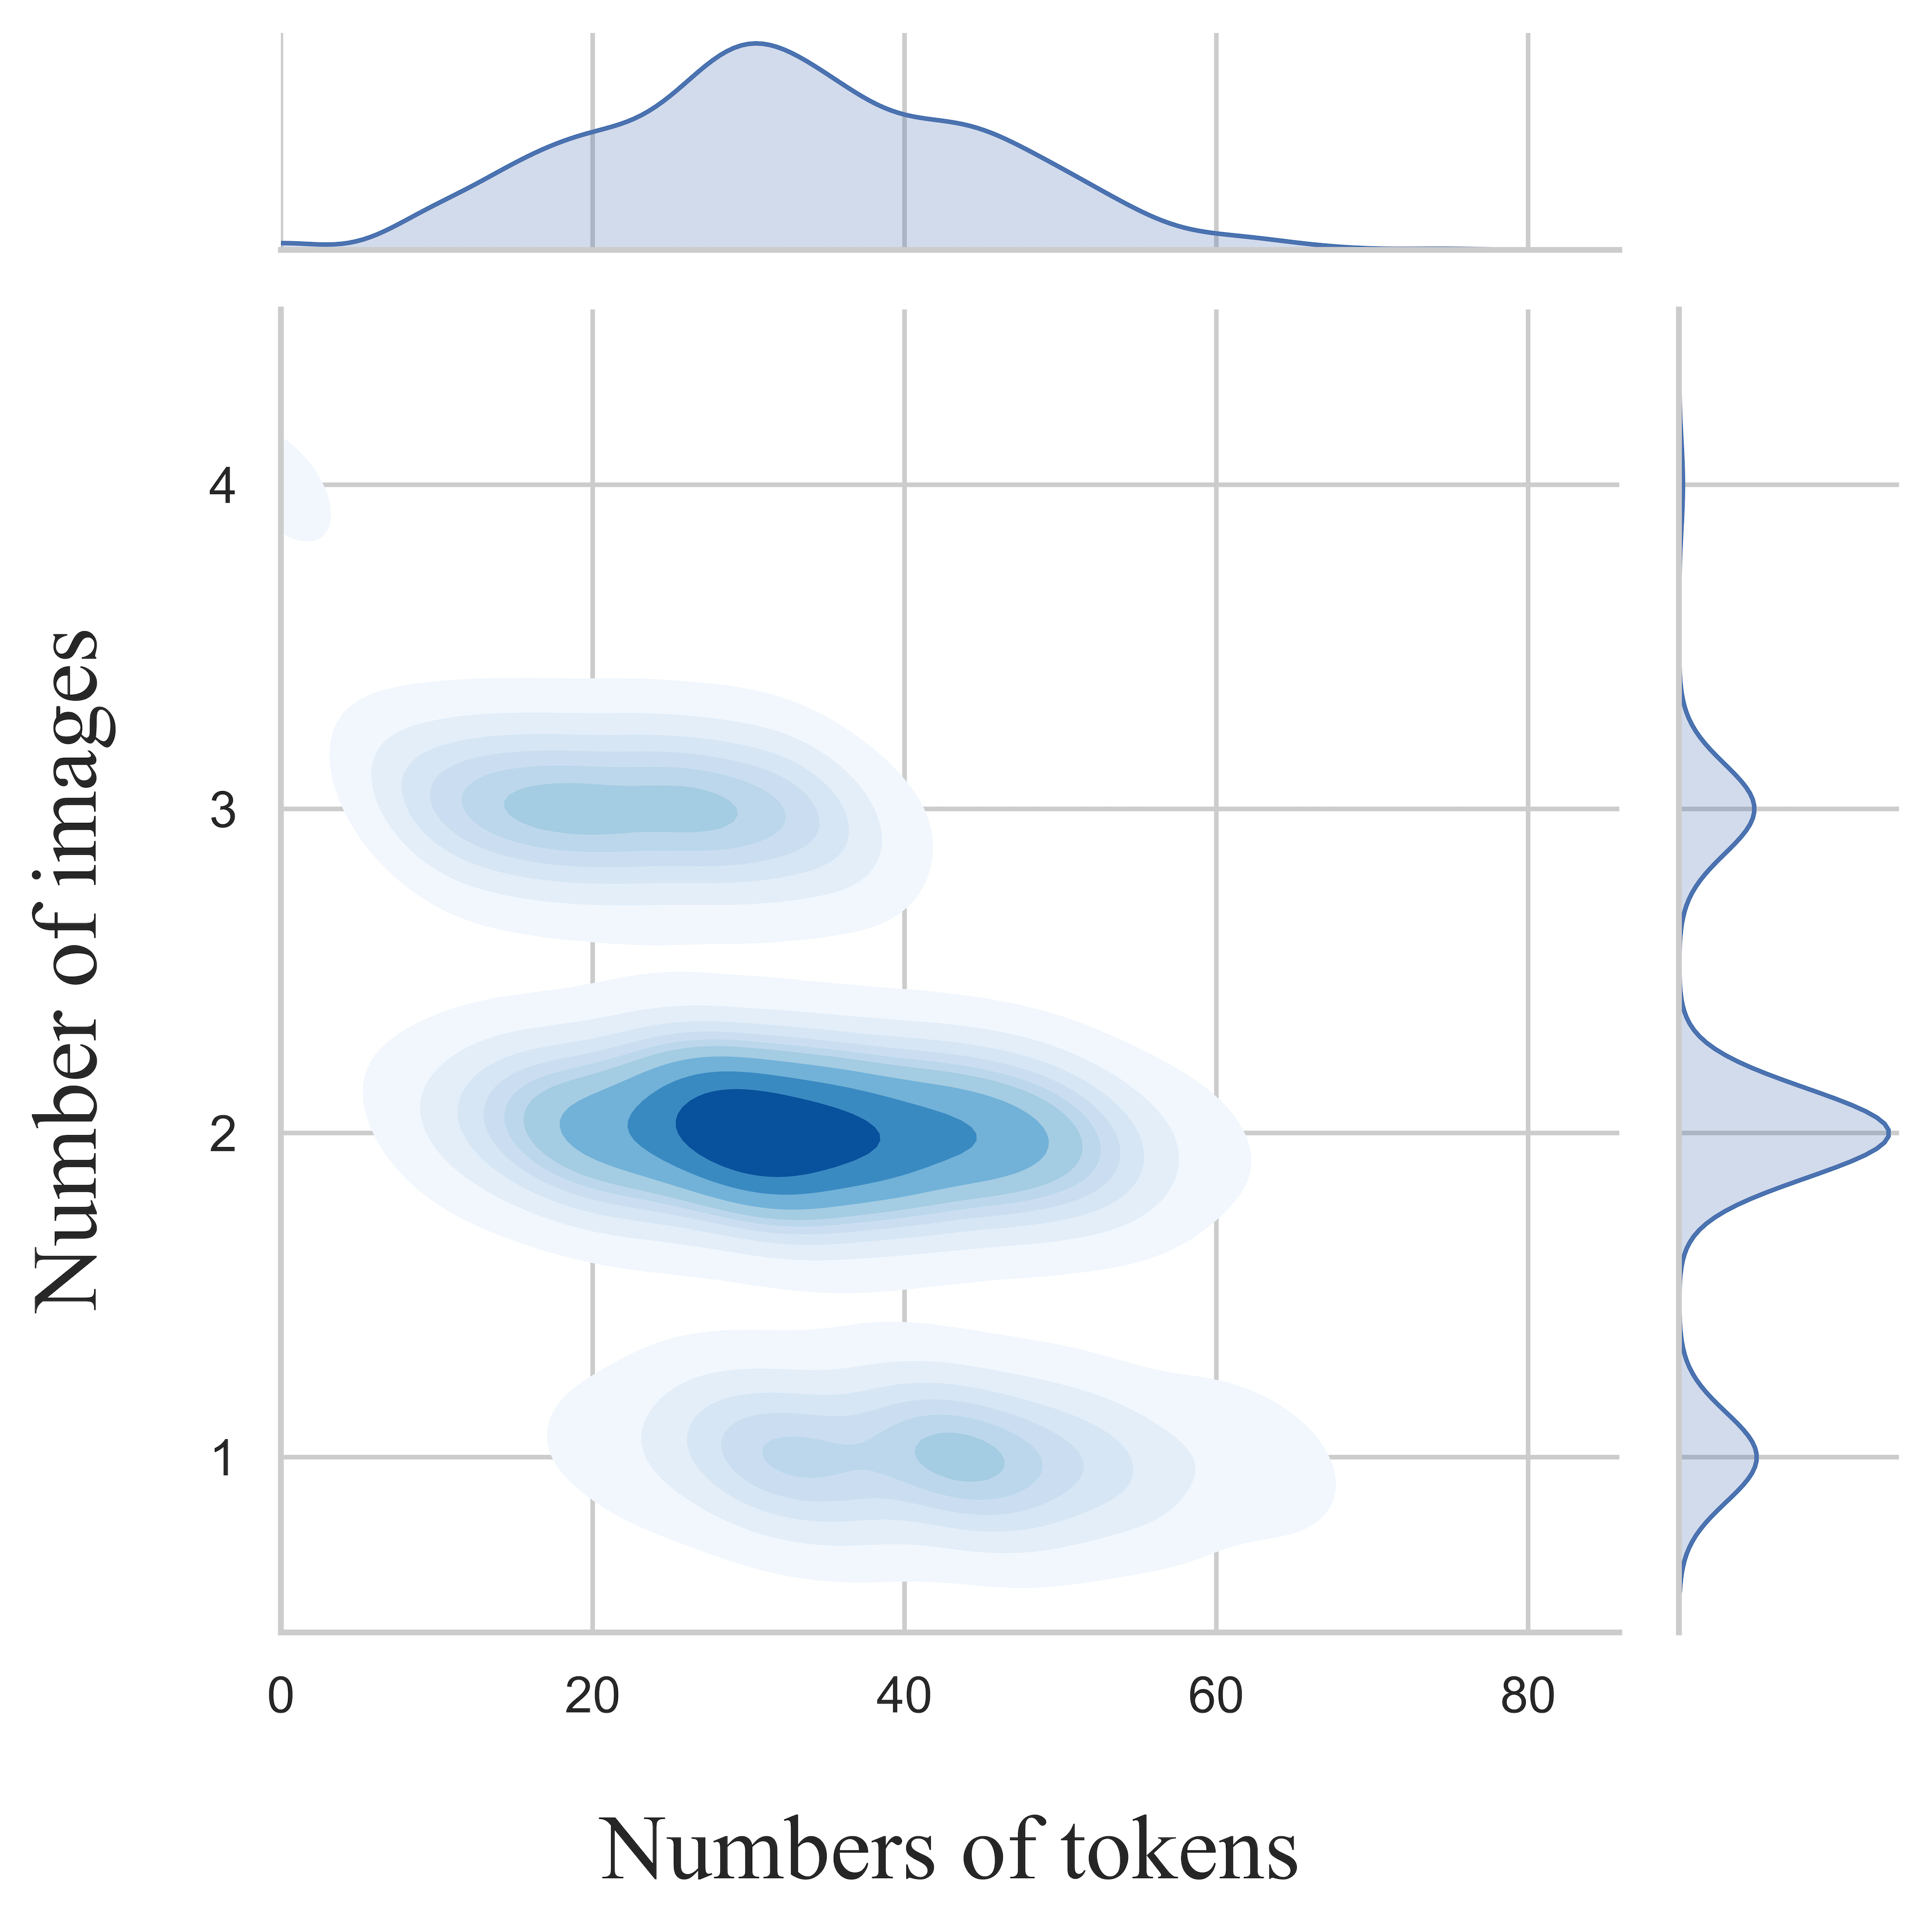
\includegraphics[width=\linewidth]{figures/src/token_img_obelics.png}
%     \caption{
%     \textbf{Joint Distribution of Text Tokens and Image Count in TextVisionBlend.} 
%     Each axis is visualized alongside the corresponding marginal distributions.
%     }
%     \label{fig:joint_distribution}
% \end{wrapfigure}


\begin{figure}
    \centering
    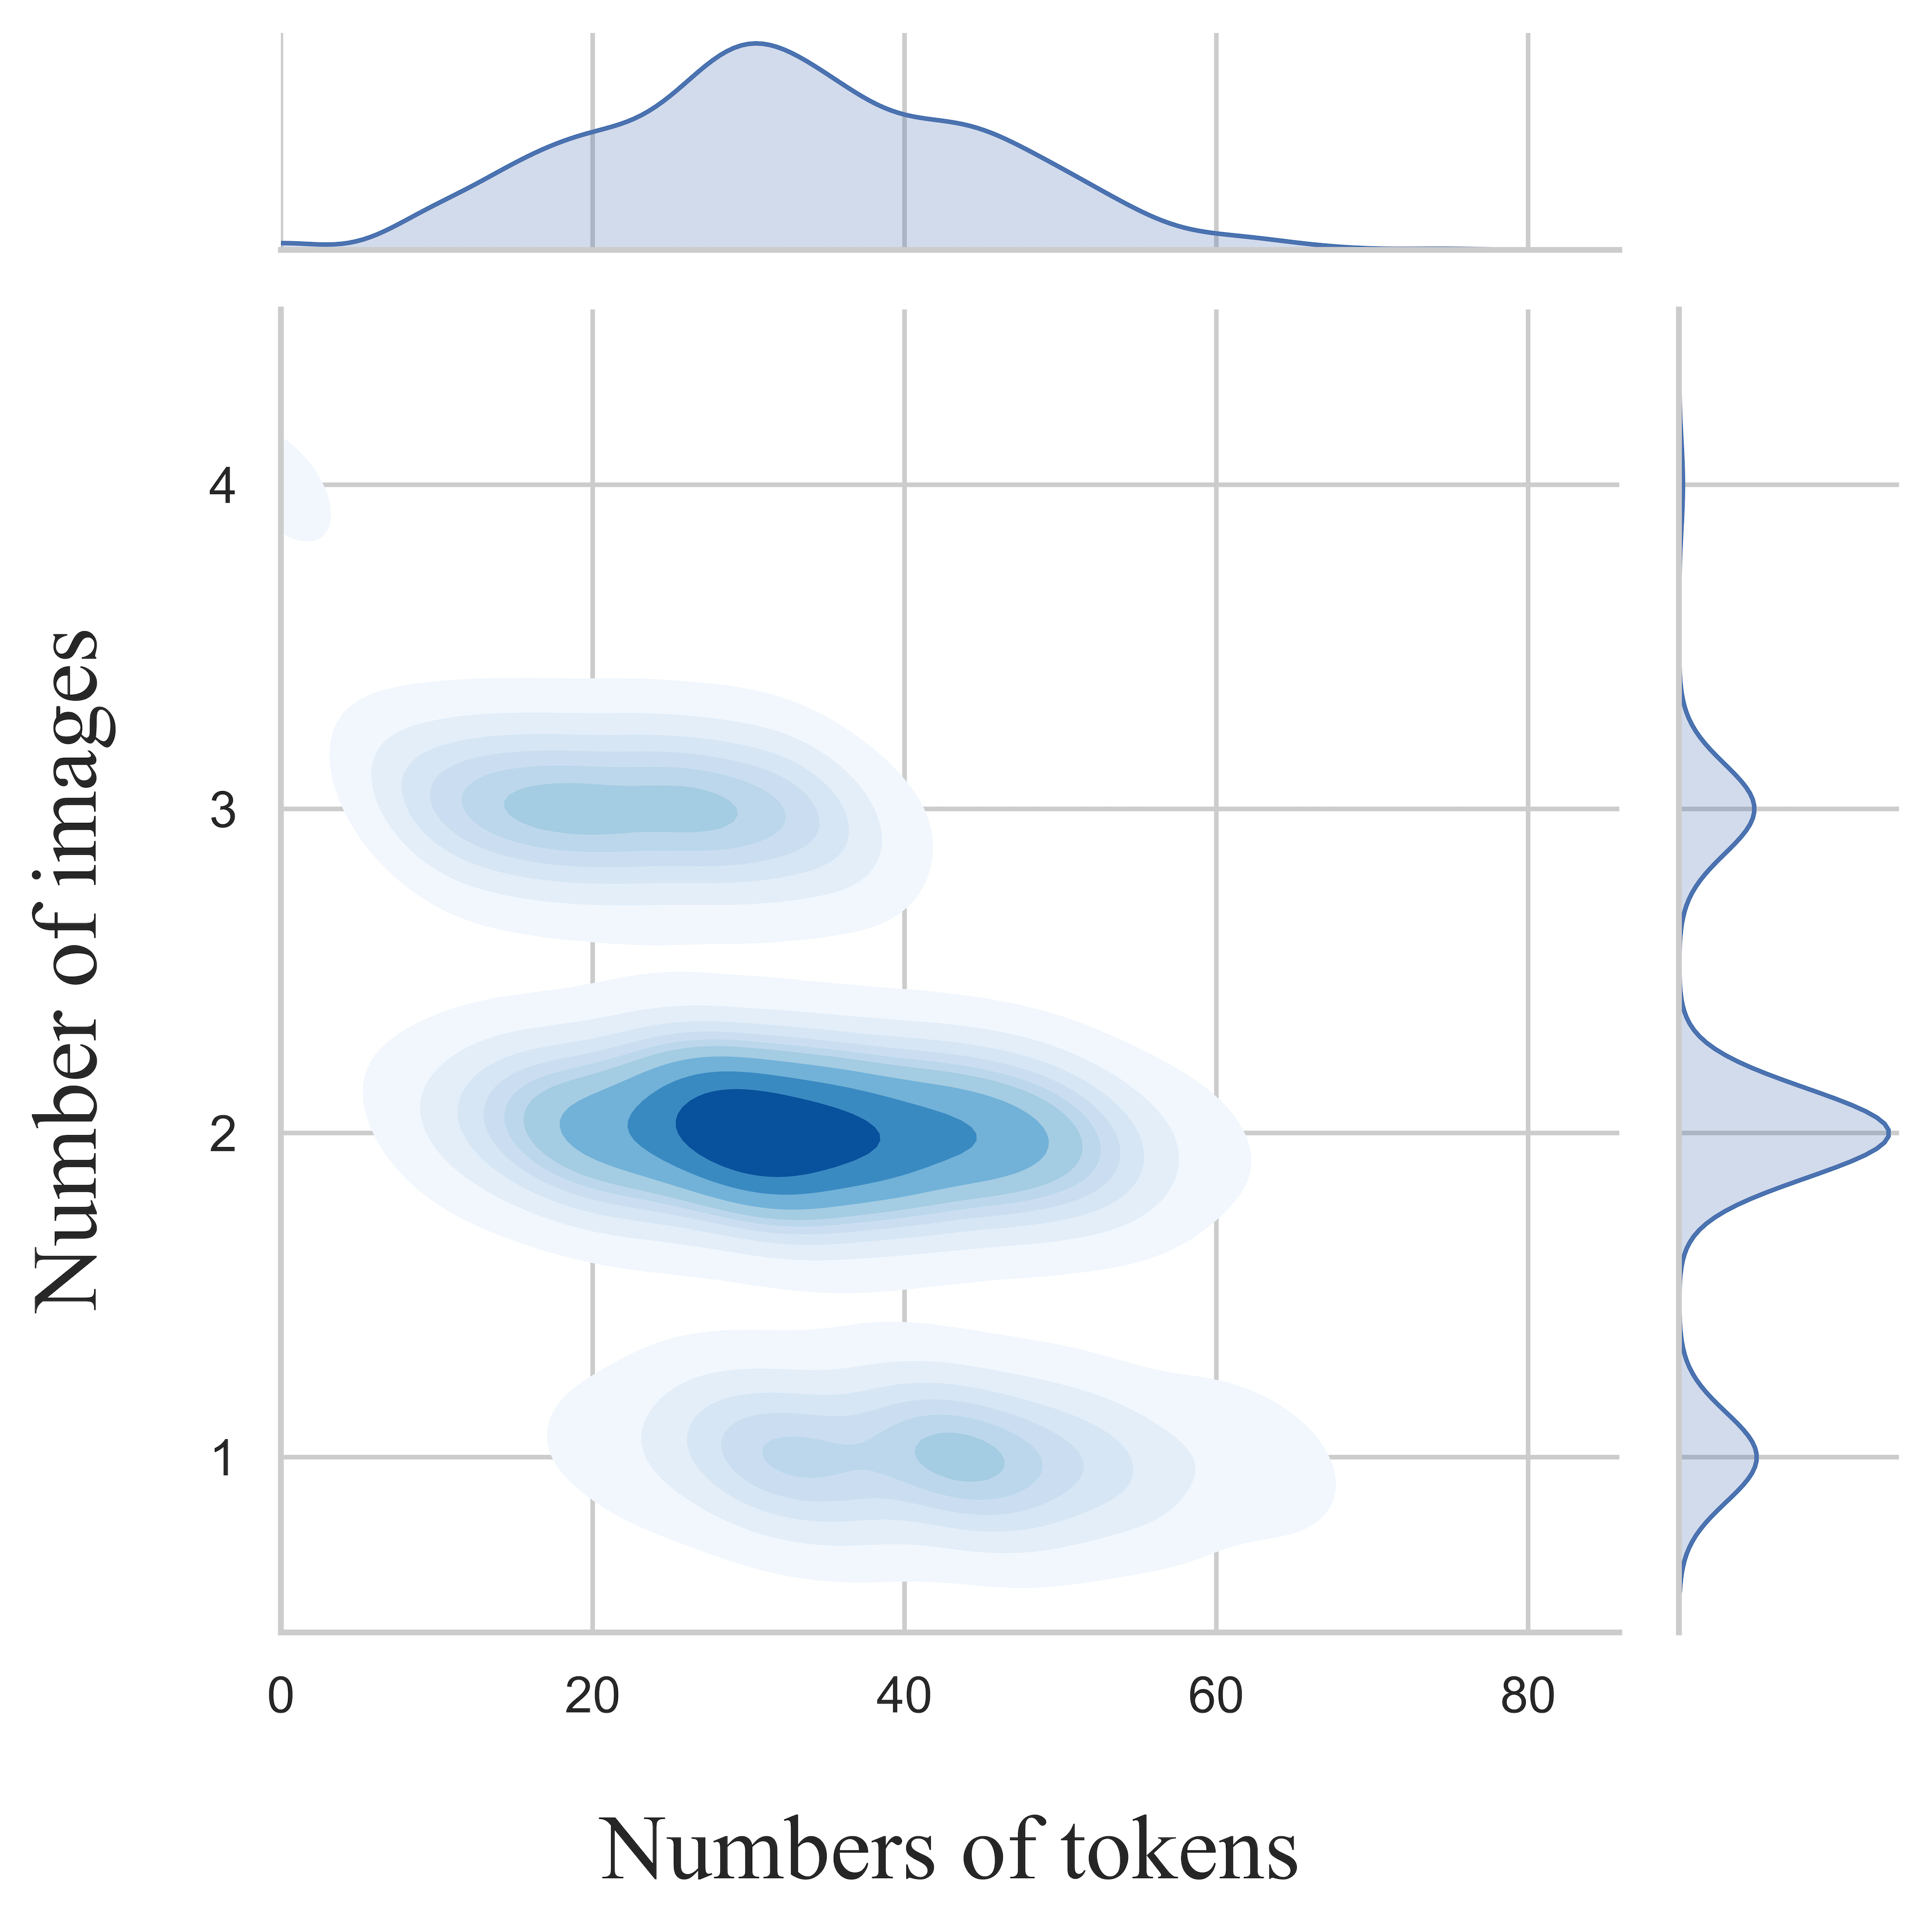
\includegraphics[width=.5\linewidth]{figures/src/token_img_obelics.png}
    % \vspace{-2mm}
    \caption{
    \textbf{Joint Distribution of Text Tokens and Image Count in TextVisionBlend.} 
    Each axis is visualized alongside the corresponding marginal distributions.
    }
    \label{fig:joint_distribution}
\end{figure}
\subsection{Joint Distribution of TextVisionBlend} Figure~\ref{fig:joint_distribution} shows the joint distribution of token numbers and image numbers in interleaved data split TextVisualBlend. 
We limit the number of images in a document to 4 images for clarity. 
The documents of \DatasetName contain a median number of images of 2 and a median number of tokens of 33.


\subsection{Examples from All Subsets}

Our \DatasetName comprises a total of 10 subsets, which can be categorized into three types: \emph{i}. Images without a specific scene, \emph{ii}. Images with a specific scene, and \emph{iii}. Images with a specific scene and bounding box annotations.

\paragraph{Images without a Specific Scene.}
For simple synthetic datasets such as Paragen-2M, where the background is plain white, we generate descriptions for image creation using prompts like: \textit{"Please generate an image of xxx based on the following text: ."}

\paragraph{Images with a Specific Scene.}
This category includes images accompanied by a scene description $T$ and OCR text $O$. Using our template, we generate longer, natural descriptions by combining these elements.

\paragraph{Images with a Specific Scene and Bounding Box.}
For datasets like AutoSlideGen, ArxivPaper generation, and interleaved sample generation, bounding box annotations are provided for each element. In these cases, we utilize LLMs to summarize all elements into a coherent paragraph. Specifically, we include details such as bounding box coordinates and the text within each box.

All subset examples are visualized in Figure~\ref{fig:all_datasets_visualization_w_anno}.

% \textcolor{red}{Note: Each subset's data, especially text annotations, requires updating.}


\input{figures/list_data_type}

\subsection{Processing Methods}
For datasets that already have captions and OCR results, such as anyword3m and mario10m, we use templates generated by GPT for concatenation (as you did before). For paragen2m, which is pure text data, we use structured sentence descriptions, e.g., "a text white background image...". For autogen and interleave data, which are interleaved distributions, we list the text and image separately in bullet points, while placing the required elements (like bbox) and fonts in the corresponding context section. For midquality data, to ensure a natural integration, we generate scene captions using Qwen2-VL and require it to generate a render text placeholder <>, which is then replaced with the rendered text. High-quality data is processed by Llama3.1 to generate scene descriptions and optimize the OCR results (see section 3.2 for the concatenation method).

\subsection{All LDA Topics}
\label{sec:all_lda}

In this section, we list top 20 LDA topics of \DatasetName in Table~\ref{tab:lda_topics_full}.
Based on the topic distribution in the table, several patterns emerge:

\begin{enumerate}
    \item \textbf{High Proportion of Common Topics}: Topics such as "Position" (15.12\%), "Signs" (14.50\%), and "Colors" (13.54\%) account for a significant portion of the dataset. These themes likely reflect common real-world scenarios, such as signage, positioning of text and images, and the use of colors in visual communication.
    
    \item \textbf{Content-Related Themes}: Content-centric topics like "Content" (14.79\%), "Community" (8.29\%), and "Safety" (2.67\%) also show relatively high proportions, suggesting that the dataset includes a considerable amount of text related to information dissemination and visual design, commonly seen in advertising and informational graphics.
    
    \item \textbf{Lower Proportion of Specialized Domains}: Topics like "Products" (1.48\%), "Cloud" (0.55\%), and "Shops" (0.78\%) have smaller representations, indicating that the dataset covers fewer instances of text-image combinations related to specific industries or niche topics.
    
    \item \textbf{Use of Numbers and Symbols}: Topics related to numbers, such as "Numbers" (1.75\%) and "Symbols" (0.61\%), occupy lower proportions, possibly reflecting that numeric and symbolic content is less prevalent in the dataset, despite its importance in some contexts.
\end{enumerate}

Overall, the dataset is more focused on common visual and textual elements seen in everyday life, such as positioning, signage, and color usage, with a relatively lower emphasis on specialized topics or numeric/symbolic content.





% \subsection{Topic Modeling:}
% Following the methodology of MMC4~\cite{mmc4}, we applied Latent Dirichlet Allocation (LDA)~\cite{lda} to examine the diversity of topics in our \DatasetName. 
% LDA provides insights into the relative proportions of each topic and the most frequently associated terms.
% From these 20 topics, we selected the 10 topics with the highest proportions for detailed analysis, as presented in Table~\ref{tab:lda_topics}.
% This table highlights the dataset’s content diversity, covering topics such as Signs, Tickets, and Community. 
% Interestingly, positional information is the most prominently represented category, which highlights that our dataset contains extensive positional data, a crucial element for understanding and processing interleaved content.
% To enhance the interpretability of the results, we employed GPT-4o to generate concise topic names based on the top 20 associated words for each topic. 

\input{Appendix/tables/lda_all}



\clearpage



\section{Visualization of \DatasetName}


\subsection{Example of StyledTextSynth Samples}
To better investigate all topics included in the StyledTextSynth sample, we show the examples in Figure~\ref{fig:mq_topics}.
We mainly list Blackboard Classroom, News, Banner, Sliver Screen, Notice Board, Advertisement Board, TV Shopping, Billboard, Booklet Page, Academic Report, Alumni Profiles, Tablet Screen, Printed Paper, Cinema Poster and Packing Box.

\input{Appendix/mq_topics}



\subsection{Examples of TextScenesHQ Samples}

We present examples of topics with the largest number of samples in Figure~\ref{fig:hq_topics}. These include:  
Product Labeling, Billboard, Packing Box, Monitor, Instruction Manual, Booklet Page, Mobile Phone Screenshot, Wall Decal, Floor Poster, Game Live, OLED Display, Protest Marches, Weather Report, Noticeboard, News Show, Blackboard Classroom, Digital Display, Cinema Caption, Wayfinding Sign, Academic Report, Alumni Profiles, Banner, Clothes with Text, and Store Sign.

These topics represent text-rich scenes commonly encountered in daily life. 
By applying our carefully designed filtering rules, we have ensured that only TextScenesHQ data is preserved for rendering.


\input{Appendix/hq_topics}



% \begin{table*}[htbp]
% \centering
% \footnotesize
% \caption{Data Level, Datasets, and Annotations Overview.}
% \begin{tabular}{x{60}lllll}
% \hline
% \textbf{Data Split} & \textbf{Dataset Name} & \textbf{\#Samples} & \textbf{Annotations} & Type & Token Length \\ \hline
% \multirow{3}{*}{Synthetic Images}
%  & CleanTextSynth & 1,907,721 & Real Text & Pure Text & 70.70\\
%  & TextVisionBlend & 547,837 & Parsed json+BLIP Caption & Pure Text & 265.62\\
%  & StyledTextSynth & 426,755 & Human+ QWEN+Intern-VL&Synthetic Image &90.00\\ 

%  \hline
% \multirow{7}{*}{Real Images}
%  & PPT2Details  & 298,565 & QWEN2-VL Caption & Powerpoint Image & 121.97\\
% & PPT2Structured& 96,457 & Parsed json+QWEN2-VL Caption &Powerpoint Image& 774.67 \\
%  & LongWordsSubset-A & 266,534 & Caption + OCR & Real Image & 38.57 \\
%  & LongWordsSubset-M & 1,299,992 & Caption + OCR & Real Image & 34.07 \\
%  & Cover Book&  207,566 & Name + Author + Category &Real Image& 28.01 \\ 
%    & Paper2Text& 356,658 &PyMuPdf phrased Text & Pure Text & 28.01\\
%  & TextScenesHQ& 36,576 &Human+Llama+Qwen+GPT4o & Real Image & 120.81\\ 
%  \hline
 
% In Total & \DatasetName  & \(\sim0.5M\) & - & - & 148.82 \\ \hline
% \end{tabular}
% \end{table*}


% \usepackage{booktabs}
% \usepackage[table]{xcolor}
% \usepackage{multirow}
% \usepackage{amsmath} % for \text

% \begin{table*}[htbp]
% \centering
% \footnotesize
% \caption{Overview of Data Splits, Datasets, Annotations, and Average Token Lengths.}
% \begin{tabular}{l l r l l r}
% \toprule
% \textbf{Data Split} & \textbf{Dataset Name} & \textbf{\#Samples} & \textbf{Annotations} & \textbf{Type} & \textbf{Token Len.} \\
% \midrule
% \rowcolor[HTML]{F2F2F2}
% \multicolumn{6}{c}{\textbf{Synthetic Images}} \\
% & CleanTextSynth       & 1,907,721  & Real Text                          & Pure Text        & 70.70  \\
% & TextVisionBlend      &   547,837  & Parsed JSON + BLIP Caption         & Pure Text        & 265.62 \\
% & StyledTextSynth      &   426,755  & Human + QWEN + Intern-VL           & Synthetic Image  & 90.00  \\
% \midrule
% \rowcolor[HTML]{F2F2F2}
% \multicolumn{6}{c}{\textbf{Real Images}} \\
% & PPT2Details          &   298,565  & QWEN2-VL Caption                   & PowerPoint Image & 121.97 \\
% & PPT2Structured       &    96,457  & Parsed JSON + QWEN2-VL Caption     & PowerPoint Image & 774.67 \\
% & LongWordsSubset-A    &   266,534  & Caption + OCR                      & Real Image       & 38.57  \\
% & LongWordsSubset-M    & 1,299,992  & Caption + OCR                      & Real Image       & 34.07  \\
% & Cover Book           &   207,566  & Name + Author + Category           & Real Image       & 28.01  \\
% & Paper2Text           &   356,658  & PyMuPdf phrased Text               & Pure Text        & 28.01  \\
% & TextScenesHQ         &    36,576  & Human + LLaMA + Qwen + GPT4o       & Real Image       & 120.81 \\
% \midrule
% \multicolumn{2}{l}{\textbf{In Total}} & \textbf{\textasciitilde0.5M} & - & - & \textbf{148.82} \\
% \bottomrule
% \end{tabular}
% \vspace{1mm}
% \begin{flushleft}
% \scriptsize
% \textbf{Notes:} JSON = structured layout annotation; OCR = optical character recognition; Intern-VL, QWEN, GPT4o, etc. are multimodal captioning models. Token length indicates average number of text tokens per sample.
% \end{flushleft}
% \end{table*}

% \usepackage{booktabs}
% \usepackage[table]{xcolor}
% \usepackage{threeparttable}
% \usepackage{array}
% \usepackage{siunitx}

\renewcommand{\arraystretch}{0.95}

\begin{table*}[htbp]
\centering
\scriptsize
\caption{ Overview of \textit{\DatasetName} Subsets: Data Splits, Annotations, and Average Token Lengths.}
\vspace{1mm}
\begin{tabular}{
    >{\raggedright\arraybackslash}p{2.5cm}
    >{\raggedleft\arraybackslash}p{1.5cm}
    % S[table-format=7.0]
    >{\raggedright\arraybackslash}p{4.0cm}
    >{\raggedright\arraybackslash}p{2.0cm}
    >{\raggedleft\arraybackslash}p{1.2cm}
    % S[table-format=3.2]
}
\toprule
\textbf{Dataset Name} & {\textbf{\#Samples}} & \textbf{Annotations} & \textbf{Type} & \textbf{Token Len.} \\
\midrule

\rowcolor[HTML]{F2F2F2}
\multicolumn{5}{c}{\textbf{Synthetic Images}} \\
CleanTextSynth      & 1,907,721 & Real Text & Pure Text & 70.70 \\
TextVisionBlend     & 547,837  & JSON + Qwen2-VL Caption & Pure Text & 265.62 \\
StyledTextSynth     & 426,755  & Human + QWEN Caption & Synthetic Image & 90.00 \\

\midrule
\rowcolor[HTML]{F2F2F2}
\multicolumn{5}{c}{\textbf{Real Images}} \\
PPT2Details         & 298,565  & Qwen2-VL Caption & PowerPoint Image & 121.97 \\
PPT2Structured      & 96,457   & JSON + Qwen2-VL Caption & PowerPoint Image & 774.67 \\
LongWordsSubset-A   & 266,534  & Caption + OCR & Real Image & 38.57 \\
LongWordsSubset-M   & 1,299,992 & Caption + OCR & Real Image & 34.07 \\
Cover Book          & 207,566  & Name + Author + Category & Real Image & 28.01 \\
Paper2Text          & 356,658  & PDF Text & Pure Text & 847.85 \\
TextScenesHQ        & 36,576   & Human + LLaMA + Qwen + GPT4o & Real Image & 120.81 \\

\midrule
% \rowcolor[HTML]{FAFAFA}
\rowcolor[HTML]{F2F2F2}
\multicolumn{5}{c}{\textbf{In Total}} \\
\multicolumn{1}{l}{\textbf{\DatasetName}} & {\textbf{\textasciitilde5M}} & \textemdash & \textemdash & \textbf{148.82} \\
\bottomrule
\end{tabular}

\vspace{1mm}
\end{table*}





\section{Annotation Quality and Error Analysis}

Automatic annotations generated by large language models (LLMs) or large vision-language models (LVMs) may introduce potential noise. 
To mitigate this, we applied systematic quality control and calibration mechanisms across different subsets of our dataset, as detailed below.

\paragraph{TextAtlasEval.}  
Every sample underwent manual verification, covering both the caption and downstream annotations. 
Samples with inaccurate or ambiguous captions were re-annotated by human annotators to ensure consistency and correctness.

\paragraph{StyledTextSynth (training set).}  
Since the text content is directly rendered into the image, OCR annotations are guaranteed to be 100\% accurate. 
However, bounding boxes may shift due to layout distortion. 
To address this, we double-checked all annotation templates and manually corrected hard cases to ensure spatial precision.

\paragraph{TextScenesHQ (training set).}  
To avoid bias from a single model, we employed both Qwen-VL and InternVL to generate annotations. 
Samples with inconsistent outputs were flagged for manual review. 
We also performed manual template filtering to maintain high quality for short-text image pairs.

\paragraph{Multi-step Calibration.}  
Our quality pipeline integrates human-in-the-loop correction, template validation, and cross-model consistency checks. 
These strategies ensure annotation reliability across key subsets including \textit{CoverBook}, \textit{CleanTextSynth}, \textit{TextVisionBlend}, \textit{StyledTextSynth}, and \textit{TextScenesHQ}. 
We will further include annotation quality statistics in the Appendix to provide transparency.

\paragraph{PPT2Details, PPT2Structured, and Paper2Text.}  
For these subsets, annotations are extracted from original PDF files using PyMuPDF. 
Since structural information such as element positions is derived directly from the source, these annotations are highly accurate. 
LLMs are only used to generate image captions and summary sentences, where they are particularly well-suited, thus introducing minimal error.

\paragraph{LongWordsSubset.}  
This subset does not rely on human annotations or LLMs. 
Instead, it is constructed by filtering existing datasets based on length and layout heuristics, ensuring high quality at scale with minimal noise.

\medskip
In summary, the combination of manual verification, template validation, and cross-model consistency checks provides robust safeguards against annotation errors. 
These procedures ensure that our dataset maintains high annotation quality across both training and evaluation splits.




\paragraph{Dataset Construction.}  
For subset TextScenesHQ of our dataset, we used GPT-4o to generate a small collection of seed topics that guided subsequent data curation.  
In addition, multimodal models such as Qwen2-VL were employed to produce descriptive annotations for image-containing subsets (e.g., \textit{PPT2Details}), where visual and textual elements had to be summarized into coherent descriptions.  
These model-generated annotations were further calibrated with template rules and human verification to ensure quality and consistency.  

\paragraph{Benchmark Evaluation.}  
To assess the reliability of our proposed benchmark, we used state-of-the-art models such as GPT-4o, Grok3, and Qwen2-VL as evaluation agents.  
These systems provided OCR-based recognition results and performance baselines against which open-source models were compared.  
This usage was strictly limited to evaluation purposes and does not affect the integrity of dataset construction.  


\medskip
Beyond the above cases, no other use of LLMs was involved in data generation, experimental design, or analysis. 


% \section{Broader impacts.}
% \textbf{Positive Impacts}:
% \DatasetName\ fills a critical gap by offering large-scale, high-quality supervision for generating images that contain paragraphs, tables, and other dense textual layouts. Models fine-tuned on it could power next-generation design aids, automatically lay out multilingual posters, or create easy-to-update infographics—lowering the barrier for small businesses, educators, and accessibility tools that convert textual content into visually engaging formats.
% \textbf{Benchmarks that reveal failure modes.} Because \EvalDatasetName\ stresses realistic layout, font, and semantic correctness, it exposes errors (e.g.\ glyph hallucination, truncation, misleading word order) that standard short-prompt benchmarks overlook. Publishing such diagnostics should steer the community toward safer, more reliable generation techniques.

% \textbf{Negative Impacts}:
% The same fidelity that benefits design also enables malicious actors to fabricate convincing invoices, legal contracts, or propaganda flyers at scale.  
% If the underlying corpus over-represents certain languages, fonts, or cultural styles, trained models may amplify biases and marginalize low-resource scripts.  
% Moreover, pre-training and evaluation on five million images demand substantial compute, potentially emitting tens of metric tons of \mbox{CO\textsubscript{2}e} and exacerbating environmental concerns.


% \textbf{Mitigation Strategies}:
% To balance innovation with responsibility, we (i) release only licensed or synthetic imagery and provide a “do-not-train” channel for rights holders; (ii) supply datasheets, language-bias audits, and safety classifiers tailored for long-text content; (iii) embed tamper-evident, model-specific watermarks to trace misuse; (iv) report energy consumption and publish distilled checkpoints to curb redundant training; and (v) prohibit use of the dataset or derivative models for fraudulent, defamatory, or otherwise unlawful content generation.


% \subsection{Full List of Topics in Middle/High Quality Datasets}

% \textbf{Also plot the ratio of each class}



% % \section{Evaluation Details}
% % To evaluate the model.

% % \subsection{Prompt Implementation.}

% x\input{tables/dataset_captions}

% \input{figures/dataset_visualization}



